We consider a simpler system to give insight into the more complex two dimensional Stommel model with the following one-dimensional model

\begin{equation}\label{eq:oneD_canonical}
\begin{aligned}
\dot{x}=-\mu+2|x|&-x|x|+A\sin(\Omega t),\\
\dot{\mu}=&-\epsilon,
\end{aligned}
\end{equation}

\begin{equation*}
x(0)=x^0,\quad\mu(0)=\mu^0,
\end{equation*}

where the constants are the slow variation rate of $\epsilon \ll 1$, the amplitude of oscillation $A$ and the frequency of oscillation $\Omega$. We also assume the initial conditions to be ${x^0=1-\sqrt{1+\mu^0}}$ and $\mu^0>\mu_{ns}$ which focuses our calculations on the lower equilibrium branch where $x<0$ and study nearby behavior.\\
The system \eqref{eq:oneD_canonical} is generalized from a basic model that contains both a smooth and non-smooth saddle-node bifurcation. This structure is similar to the Stommel model and hence a good model to test features like slow variation or oscillatory forcing. In each case, emphasis is put on the non-smooth component of the model to study the non-smooth bifurcation and the role it plays in the hysteresis curve we anticipate in the Stommel model.

\section{Static Bifurcations}
\label{sec:oneD_static}

The foundation to our understanding comes from the simplest structure lying within the canonical system \eqref{eq:oneD_canonical} which is the bifurcation structure. This means finding the general form for the equilibria in \eqref{eq:oneD_canonical} with $A=0$ and $\epsilon=0$, which is our basic model with a static $\mu$ and no forcing. As we have a fixed parameter value, we search for a point or set of points that the solution relaxes to as $t\to \infty$. We call these points the equilibrium points and they are either stable or unstable equilibria. But as we are considering all possible $\mu$, we want all of the equilibrium points for each $\mu$ and thus we call these the equilibrium branches.

To find all equilibrium branches, we search for when the solution has come to a rest, which is equivalent to setting the derivative of $x$ is zero. Thus we set \eqref{eq:oneD_canonical} to zero with

\begin{equation}\label{eq:oneD_static_equil}
0=-\mu +2|x|-x|x|.
\end{equation}

Solving \eqref{eq:oneD_static_equil} results in 3 solutions, the stability of each is characterized by small perturbations to the equilibrium linearly growing or decaying. We denote the stable equilibria as $x_l$ and $x_u$ for the lower and upper branches respectfully, and a single unstable middle branch, $x_{m}$. These are

\begin{equation*}
x_l=1-\sqrt{1+\mu},\quad x_u=1+\sqrt{1-\mu},\quad
x_{m}=1-\sqrt{1-\mu}.
\end{equation*}

We note that $x_l$ is valid for $\mu\ge 0$ and both $x_u$ and $x_{m}$ for $\mu\le 1$. Thus this system has a stable equilibrium for each value of the parameter and has a region of bi-stability for $0\le \mu\le 1$. The boundary of this region are bifurcations at the points ${(\mu_{ns},x_{ns})=(0,0)}$ and $(\mu_{\text{smooth}},x_{\text{smooth}})=(1,1)$ which are the non-smooth and smooth saddle-node bifurcations respectfully. Both are of saddle-node type due to pairs of equilibria annihilating at these locations. This is shown in figure~\ref{fig:oneD_static_bifdiagram}.

\begin{figure}[H]
\centering
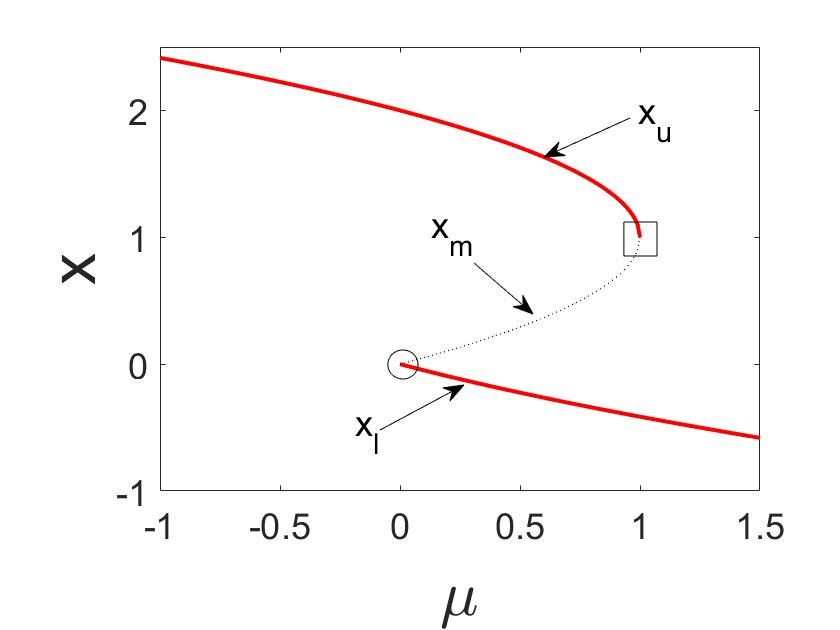
\includegraphics[width=.8\textwidth]{oneD/bif_diagram.jpg}
\caption{The one-dimensional bifurcation diagram with the upper and lower equilibrium branches as well as the unstable middle branch. The non-smooth bifurcation occurs at (0,0) with the circle and the smooth bifurcation occurs at (1,1) with the box. }
\label{fig:oneD_static_bifdiagram}
\end{figure}


\section{Slowly Varying Bifurcation Parameter}
\label{sec:oneD_slow}

To develop a method for the slowly varying Stommel model, we consider \eqref{eq:oneD_canonical} with $\epsilon\ll 1$ and $A=0$. Under these conditions, $\mu(t)$ is a function of time and thus a bifurcation no longer occurs. Instead, it is expected that a tipping point occurs nearby the static bifurcation points as long as $\epsilon$ is small. The smooth case is well understood, see \cite{zhu2015tipping}, so we consider the behavior of the non-smooth bifurcation with $x<0$. From \cite{haberman1979slowly} as well as the smooth problem \cite{zhu2015tipping}, it is common practice to rescale time in a model to put the dynamics on the same order and allow for algebraic solutions to be found. Here we have the parameter $\mu(t)$ is slowly varying in time so it makes sense to rescale using this as our 'slow' time, $\tau=\epsilon t$. Applying both $x<0$ and this 'slow' time approach to the system \eqref{eq:oneD_canonical} then gives

\begin{equation}\label{eq:oneD_slow_scaled}
\begin{aligned}
\epsilon x_\tau=&-\mu(\tau)-2x+x^2,\\
\mu_\tau=&-1.
\end{aligned}
\end{equation}

A standard approach to extracting information out of complicated models is to try to find reduced equations by separating the behavior at each order. This approach is known as using an asymptotic expansion and further details can be found in Murray's \textit{Asymptotic Analysis} \cite{murray2012asymptotic}. With $\epsilon$ being the small quantity that dictates our 'slow' time, we choose to use an asymptotic expansion of $x$ with

\begin{equation}\label{eq:oneD_slow_asympexpan}
x(\tau)\sim x_0(\tau)+\epsilon x_1(\tau)+\epsilon^2 x_2(\tau)+O(\epsilon^3).
\end{equation}

This approach captures the slowly varying behavior of the solution in terms of this small quantity $\epsilon$ and aims to relate the slow variation to the solution. We substitute the expansion \eqref{eq:oneD_slow_asympexpan} into the scaled system \eqref{eq:oneD_slow_scaled} to get

\begin{equation*}
\epsilon {x_0}_\tau +\epsilon^2 {x_1}_\tau+\ldots= -\mu(\tau) -2x_0+x_0^2+\epsilon(-2x_1+2x_1x_0)+\epsilon^2(-2x_1+2x_2x_0+x_1^2)+\ldots
\end{equation*}

Once we separate the equations at each order of $\epsilon$, we find the following system of equations

\begin{align}
\label{eq:oneD_slow_outerO1}
O(1):& \quad 0=-\mu(\tau)-2x_0+x_0^2,\\
\label{eq:oneD_slow_outerO2}
O(\epsilon):& \quad 0=-{x_0}_\tau-2x_1+2x_1 x_0,\\
\label{eq:oneD_slow_outerO3}
O(\epsilon^2):& \quad 0=-{x_1}_\tau-2x_2+2x_2x_0+x_1^2.
\end{align}

Each of the equations \eqref{eq:oneD_slow_outerO1}-\eqref{eq:oneD_slow_outerO3} gives the respective order's pseudo-equilibrium. Thus we sole each progressively to find the terms of our asymptotic expansion \eqref{eq:oneD_slow_asympexpan} as

\begin{equation}\label{eq:oneD_slow_outersoln}
x(t)\sim 1-\sqrt{1+\mu(t)}+ \frac{\epsilon}{4(1+\mu(t))}-\frac{3\epsilon^2}{32(1+\mu(t))^{5/2}}+O(\epsilon^3).
\end{equation}

We call \eqref{eq:oneD_slow_outersoln} the outer solution as it approximates the solution well for values of $x(t)$ away from the bifurcation value $\mu_{ns}$. But since the dynamics of the system \eqref{eq:oneD_canonical} change at $x=0$ due to the non-smooth bifurcation of the underlying static system, this solution is valid only for $x<0$ and $\mu>0$.


It is a key assumption of an asymptotic expansion that the terms are clearly separated by order of $\epsilon$. We observe a scaling of $\mu$ and $x$ for which \eqref{eq:oneD_slow_outersoln} is no longer valid under this assumption of order separation, here when $x_0\sim \epsilon x_1$, which occurs for $\mu\sim O(\epsilon)$. We conduct a simple scale analysis to determine the appropriate scaling for the local analysis about $x=0$. Hence we consider the general scales

\begin{equation*}
x=\epsilon^\alpha y,\quad \mu = \epsilon^\beta m,
\end{equation*}

with $\alpha>0$ and $\beta>0$ for an inner scaling. We apply this scaling in \eqref{eq:oneD_canonical} to give the system

\begin{equation}\label{eq:oneD_slow_scalesearch}
\begin{aligned}
\epsilon^\alpha \dot{y}=&-\epsilon^\beta m +\epsilon^\alpha 2|y|-\epsilon^{2\alpha}y|y|,\\
 \epsilon^\beta \dot{m}=&-\epsilon.
\end{aligned}
\end{equation}

We balance the leading order terms $\epsilon^\alpha\dot{y}$ with $\epsilon^\beta m$ to give $\alpha=\beta$. But the equation for $m$ calls for $\beta=1$, thus we have the scaling for the local analysis

\begin{equation}\label{eq:oneD_slow_scales}
x=\epsilon y,\quad \mu=\epsilon m.
\end{equation}

We have found that the scalings in \eqref{eq:oneD_slow_scales} apply to all $x$ and thus we consider the region of $x>0$. Substituting the local variables \eqref{eq:oneD_slow_scales} into the original model \eqref{eq:oneD_canonical} we find the following inner system for the region of $x>0$

\begin{equation}\label{eq:oneD_slow_innereq}
\begin{aligned}
\dot{y}=&-m(t)+2 y-\epsilon y^2,\\
\dot{m}=&-1.
\end{aligned}
\end{equation}

We recall that we are searching for a link between $y$ and $m$, and from \cite{haberman1979slowly} we use that it is then convenient to change the differentiation on $y$ to be with respect to the parameter $m$. This incorporates the behavior of $m(t)$ directly into the equation we solve and gives us a direct method for finding the tipping point. Then the leading order equation is

\begin{equation}\label{eq:oneD_slow_innerm}
y_m = m-2y.
\end{equation}

The leading order solution to \eqref{eq:oneD_slow_innerm} is found explicitly as follows

\begin{equation*}
y(m) = C e^{-2m}+\frac{m}{2}-\frac{1}{4}+O(\epsilon).
\end{equation*}

With the inner solution found in terms of the parameter $m$, we write this in terms of the original coordinates with

\begin{equation}\label{eq:oneD_slow_innersoln}
x(t)\sim Ce^{-2\mu(t)/\epsilon}+\frac{\mu(t)}{2}+O(\epsilon).
\end{equation}

Since the solution \eqref{eq:oneD_slow_innersoln} behaves exponentially, the tipping point, $\mu_{\text{slow}}$, occurs when the exponential term begins to grow rapidly. Here we consider tipping to occur when the solution becomes $O(1/\epsilon)$. Thus we find the tipping point $\mu_{\text{slow}}$ to take the form

\begin{equation}\label{eq:oneD_slow_tipping}
\mu_{\text{slow}}= \frac{1}{2}\epsilon \log (\epsilon).
\end{equation}

Thus we have the tipping point for the purely smooth one-dimensional model. Notice that for small values of $\epsilon$, the slowly varying parameter causes tipping to occur when $\mu(t)<0$, which is after the non-smooth bifurcation and is consistent with considering the inner equation \eqref{eq:oneD_slow_innereq} for the region $x>0$ as we found in the analysis. Thus we find that a slow varying bifurcation parameter causes a delay in the rapid transition to the upper branch and we expect the solution to remain near the lower branch for longer than in the static problem. In terms of hysteresis, then slow variation allows for a longer period before the states switch from the lower branch to the upper.

In figure~\ref{fig:oneD_slow_numerics} (a,b), an example of this tipping is shown for a choice in $\epsilon$ along with the standard bifurcation diagram where (c) demonstrates the tipping approximation across a range of $\epsilon$. The concavities match as well as clear agreement in the estimation of the tipping point as $\epsilon$ goes to 0.

\begin{figure}[H]
\centering
\begin{subfigure}{.5\textwidth}
 \centering
 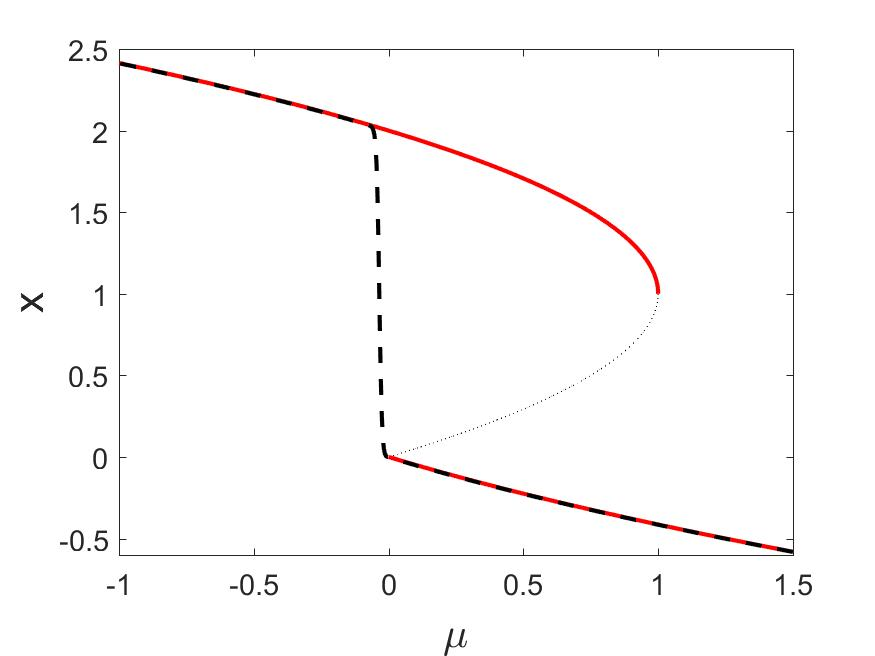
\includegraphics[width=\linewidth]{oneD/slow_bif_diagram.jpg}
 \caption{}
\end{subfigure}%
\begin{subfigure}{.5\textwidth}
 \centering
 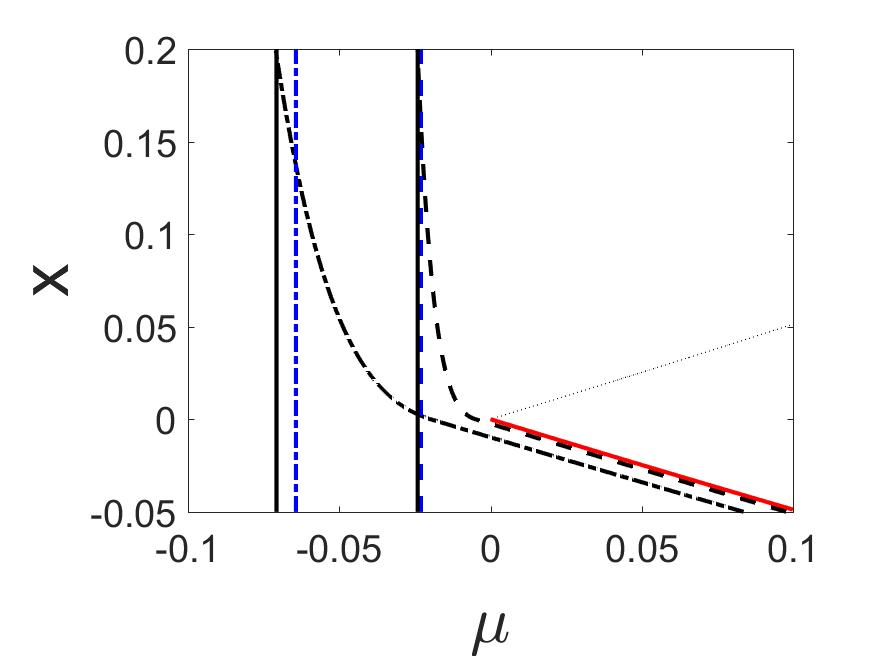
\includegraphics[width=\linewidth]{oneD/slow_bif_diagram_zoom.jpg}
 \caption{}
\end{subfigure}
\begin{subfigure}{.5\textwidth}
\centering
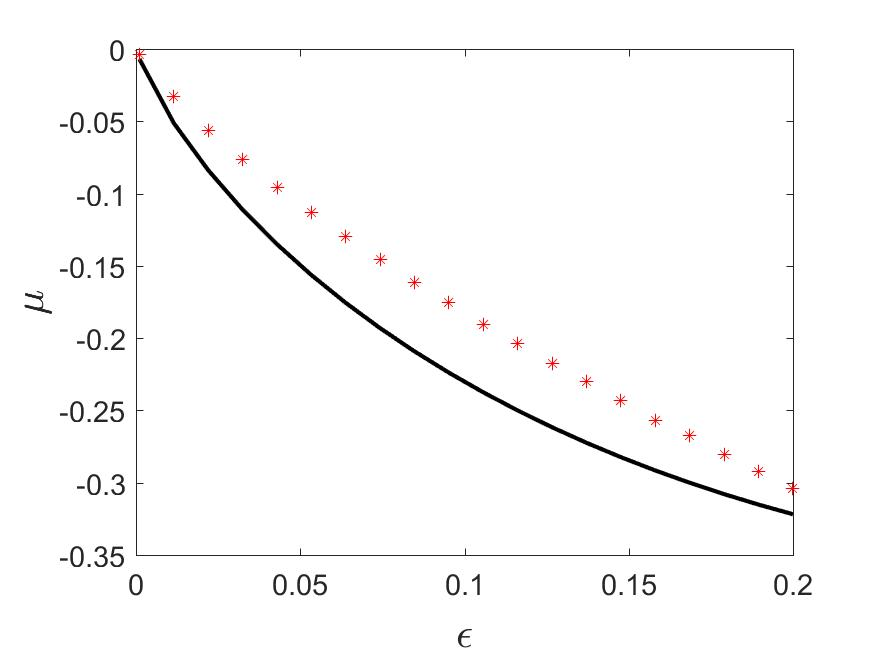
\includegraphics[width=\linewidth]{oneD/slow_epscomp.jpg}
\caption{}
\label{fig:oneD_slow_comp}
\end{subfigure}
\caption{In (a) the numerical solution (black dotted line) to \eqref{eq:oneD_canonical} is given with $A=0$ and $\epsilon=.01$. The bifurcation plot is overlayed for convenience. In (b) a zoom in of what happens near the non-smooth bifurcation. The solid vertical line (black) is the numerical tipping which we use the criteria $x>.5$ and the dotted vertical line (blue) is the tipping estimate. In (c) a range of $\epsilon$ and their corresponding tipping (red stars) are compared to our estimate (solid black line) from \eqref{eq:oneD_slow_tipping}.}
\label{fig:oneD_slow_numerics}
\end{figure}


\subsection{Stability}
From the static model we know our outer solution \eqref{eq:oneD_slow_outersoln} to be stable, but to verify that the inner solution \eqref{eq:oneD_slow_innersoln} is stable, we use a simple linear stability analysis on the inner system. Typically to do this, an analysis would be performed about an equilibrium to see if perturbations would grow or decay. But as this problem has a parameter that is allowed to vary, we instead must be careful to note the analysis must be done on the pseudo-equilibrium instead. In the first region of interest, $m(t)\ge 0$, the following inner equation and pseudo-equilibrium hold below the axis

\begin{equation}\label{eq:oneD_slow_stability1}
\dot{y}=-m(t)-2y=f(t,y), \quad z^0(t)=-\frac{m(t)}{2}.
\end{equation}

We then consider simple perturbations about the pseudo-equilibrium in \eqref{eq:oneD_slow_stability1} with

\begin{equation*}
y(t)=z^0(t)+u(t), \quad \lVert u(t) \rVert \ll 1.
\end{equation*}

Normally a Taylor expansion would result in expressing the perturbations with their own equation that we could use to determine stability. Since $z^0(t)$ isn't fixed, we must consider its contribution to the derivative in this region of the parameter space (i.e $m(t)\ge 0$). Thus we find

\begin{equation}\label{eq:oneD_slow_stability2}
\begin{aligned}
\dot{y} =& \dot{z}^0+\dot{u},\\
\dot{z}^0= & \begin{cases}
\frac{1}{2} & m(t)>0,\\
0 & m(t)=0.
\end{cases}
\end{aligned}
\end{equation}

Now we apply the standard Taylor expansion to see the behavior of these perturbations and with the contributions in \eqref{eq:oneD_slow_stability2}, the inner equation \eqref{eq:oneD_slow_stability1} becomes

\begin{equation}\label{eq:oneD_slow_perturbeq}
\begin{aligned}
\dot{y}=& f(t,z^0)+f_y(t,z^0)(y-z^0)
=& f_y(t,z^0)u,\\
\dot{u}=&\begin{cases}
-\frac{1}{2}-2u, & m(t)>0,\\
-2u, & m(t)=0.
\end{cases}
\end{aligned}
\end{equation}

If this were the static parameter problem, we would always have the second case in \eqref{eq:oneD_slow_perturbeq}, which is always stable due to the sign. But since we allow for a varying parameter, we learn that the solution is attracted to just below the pseudo-equilibrium $z^0(t)$. But as this system always experiences the critical point $m=0$ due to the continuous decrease in $m(t)$, the slowly varying parameter eventually acts like the static parameter in \autoref{sec:oneD_static}. Hence we have that for $x<0$, the pseudo-equilibrium is hyperbolic and asymptotically stable. But here there is a critical point at $(\mu_{ns},x_{ns})=(0,0)$ which corresponds to a non-hyperbolic equilibrium point. Generally, non-hyperbolic behavior signals equilibrium structure to be changing. Here, this signals a transition in behavior for $x>0$ and helps identify that the tipping occurs here.

For the second region of interest, $m(t)<0$, we found a solution that had the following inner equation which has the pseudo-equilibrium above the axis with

\begin{equation}\label{eq:oneD_slow_innerstability}
\dot{y}=-m(t)+2y, \quad z^0(t) = \frac{m(t)}{2}.
\end{equation}

But we find a contradiction from \eqref{eq:oneD_slow_innerstability}, here $m(t)<0$ yet the solution of this region is above the axis $x=0$. Thus we may conclude that this inner equation has no equilibrium in this region and further verifies that the critical point $(\mu_{ns},x_{ns})$ was non-hyperbolic and tipping occurs for $m(t)<0$.

\section{High Frequency Oscillatory Forcing}
\label{sec:oneD_highfreqosc}

To understand the oscillatory forcing in the Stommel model, consider the canonical system \eqref{eq:oneD_canonical} with $A\sim O(1)$, $\Omega\gg 1$ and $\epsilon=0$, which gives purely high frequency oscillatory forcing in the system. Under these conditions, we have a static parameter and for each parameter value there is oscillatory forcing with solutions characterized by oscillations about a fixed point. Thus we should expect to find a bifurcation influenced by oscillations occurring under these conditions. Here we develop a method to find oscillatory solutions to determine what the effect of oscillatory forcing has on the bifurcation of \eqref{eq:oneD_canonical}. Where \autoref{sec:oneD_slow} focused only on the slowly varying dynamics, here we have both a 'slow' time scale $t$ and a 'fast' time scale $T=\Omega t$. This naturally suggests a multiple scales approach where we search for a solution that is dependent on both of these scales, $x(t)=x(t,T)$. This method is commonly used in problems that have behavior observable on multiple scalings, and we use it here to find a way to accurately analyze each scale and effectively combine their behavior into a single unifying solution. Further discussion on this method can be found in \cite{sanchez1996method}.

Recall that our focus is on the non-smooth behavior and hence we restrict the solution to follow along the lower stable equilibrium branch where $x<0$. Using this multiple scales approach, our canonical system \eqref{eq:oneD_canonical} has the following form

\begin{equation}\label{eq:oneD_osc_multiscale}
x_T+\Omega^{-1}x_t=\Omega^{-1}\left(-\mu-2x+x^2+A\sin(T)\right).
\end{equation}

In \eqref{eq:oneD_osc_multiscale}, the small quantity $\Omega^{-1}$ appears which suggests an asymptotic expansion in powers of this quantity

\begin{equation}\label{eq:oneD_osc_asymptotic}
x(t,T)\sim x_0(t,T)+\Omega^{-1}x_1(t,T)+\Omega^{-2}x_2(t,T)+O(\Omega^{-3}).
\end{equation}

Substituting \eqref{eq:oneD_osc_asymptotic} into \eqref{eq:oneD_osc_multiscale}, we find

\begin{equation*}
{x_0}_T+\Omega^{-1}{x_0}_t+\Omega^{-1}{x_1}_T+\ldots=\Omega^{-1}(-\mu-2x_0+x_0^2+A\sin(T))+\Omega^{-2}(-2x_1+2x_1x_0)+\ldots
\end{equation*}

Here we separate the reduced equations at order of $\Omega$ to get

\begin{align}
\label{eq:oneD_osc_outerO1}
O(1):& \quad {x_0}_T=0, \\
\label{eq:oneD_osc_outerO2}
O(\Omega^{-1}):& \quad {x_1}_T+{x_0}_t =-\mu-2x_0+x_0^2+A\sin(T),\\
\label{eq:oneD_osc_outerO3}
O(\Omega^{-2}):& \quad {x_2}_T + {x_1}_t= -2x_1+2x_0 x_1.
\end{align}

With an equation at each order, we must able to solve each to proceed to the next but we must also further restrict our solution from having resonant or linearly growing terms to prevent any multiplicity or exponential growth. This assures that the terms in the asymptotic expansion are compatible with one another and we find a robust solution. A common method to guarantee compatible solutions with sublinear growth at each order is the Fredholm alternative. This provides a solvability condition for each equation of the form ${x_i}_T=R_i(t,T)$ with

\begin{equation*}
\lim\limits_{T\to\infty}\frac{1}{T}\int_0^T R_i(t,u)\,du=0,
\end{equation*}

although for this system we consider the periodic form of the Fredholm alternative

\begin{equation} \label{eq:Fredholm}
\frac{1}{2\pi}\int_0^{2\pi}R_i(t,T)\,dT=0.
\end{equation}

Both the general and periodic form of the Fredholm alternative have been well studied and a more theoretic approach to the periodic version is discussed in Bensoussan's \textit{Asymptotic analysis for periodic structures} \cite{bensoussan2011asymptotic}. From \eqref{eq:oneD_osc_outerO1}, we learn the leading order term is only dependent on the 'slow' time, $x_0=x_0(t)$. Applying the Fredholm alternative \eqref{eq:Fredholm} to \eqref{eq:oneD_osc_outerO2} gives

\begin{equation}\label{eq:oneD_osc_outerO2soln}
\begin{aligned}
0=&\frac{1}{2\pi}\int_0^{2\pi} -{x_0}_t(t) -\mu -2x_0(t)+x_0(t)^2+A\sin(T)\,dT ,\\
{x_0}_t=& -\mu -2x_0+x_0^2 ,\\
{x_1}_T =& A\sin(T).
\end{aligned}
\end{equation}

Solving for the equilibrium solution of \eqref{eq:oneD_osc_outerO2soln} leads to the leading order solution, $x_0$, and also allows us to partially solve for the first correction term $x_1$ with

\begin{equation*}
\begin{aligned}
x_0 =& 1-\sqrt{1+\mu},\\
x_1(t,T) =& v_1(t) - A\cos(T).
\end{aligned}
\end{equation*}

Repeating this procedure with \eqref{eq:oneD_osc_outerO3}, this is shown in \autoref{app:oneD}, results in the expansion \eqref{eq:oneD_osc_asymptotic} written in the original coordinates

\begin{equation}\label{eq:oneD_osc_outersoln}
x\sim 1-\sqrt{1+\mu}-\Omega^{-1} A \cos(\Omega t)+O(\Omega^{-2}).
\end{equation}

Once again, the explicit outer solution \eqref{eq:oneD_osc_outersoln} performs well for $x$ away from the bifurcation, we search for when the assumptions of the asymptotic series fail indicating where an inner analysis is needed. This is when $x_0\sim \epsilon x_1$ which occurs for $\mu\sim O(\Omega^{-1})$.

We consider a general scaling for $x=\Omega^{-\alpha}y$ and $\mu = \Omega^{-\beta}m$ where $\alpha>0$ and $\beta>0$ allows for an inner equation. Applying these scalings to \eqref{eq:oneD_canonical} results in

\begin{equation}\label{eq:oneD_osc_generalinner}
\dot{y} = -\Omega^{\alpha-\beta}m+2|y|-\Omega^{-\alpha}y|y|+\Omega^{\alpha}A\sin(\Omega t)
\end{equation}

Since $\mu$ is fixed for this section, we are still able to use the same time scales, $t=t$ and $T=\Omega t$. We also have the same assumption that $y(t)=y(t,T)$ and hence a similar multiple scales argument in \eqref{eq:oneD_osc_generalinner} leads to

\begin{equation}\label{eq:oneD_osc_innergeneralmulti}
y_T+\Omega^{-1}y_t = - \Omega^{\alpha-\beta-1}m+\Omega^{-1}2|y|-\Omega^{-\alpha-1}y|y|+\Omega^{\alpha-1}A\sin(T).
\end{equation}

With a standard balancing argument between the leading order terms in \eqref{eq:oneD_osc_innergeneralmulti}, $y_T$ and $\Omega^{\alpha-1} A\sin(T)$, we see that $\alpha=1$. But we also want to see the terms $\Omega^{\alpha-\beta-1}m$ balance with $\Omega^{-1}2|y|$, which gives us that $\beta=1$ as well. This results in the inner equation

\begin{equation}\label{eq:oneD_osc_naivemultiscales}
y_T+\Omega^{-1}y_t = \Omega^{-1}\left(-m+2|y|\right)-\Omega^{-2}y|y|+A\sin(T).
\end{equation}

Similarly to the outer equation, we approximate the solution with asymptotic expansion in terms of $\Omega^{-1}$ 

\begin{equation}\label{eq:oneD_osc_innerasymptotic}
y(t,T)\sim y_0(t,T)+\Omega^{-1}y_1(t,T)+O(\Omega^{-2}).
\end{equation}

Substituting the expansion \eqref{eq:oneD_osc_innerasymptotic} into the inner equation \eqref{eq:oneD_osc_naivemultiscales} we find

\begin{equation*}
{y_0}_T+\Omega^{-1}{y_0}_t+\Omega^{-1}{y_1}_T+\ldots =\begin{aligned}[t]\Omega^{-1}&(-m+2|y_0+\Omega^{-1}y_1+\ldots|)+A\sin(T)\\
&+\Omega^{-2}(y_0+\Omega^{-1}y_1+\ldots)|y_0+\Omega^{-1}y_1+\ldots|
\end{aligned}
\end{equation*}

Here we then find the following system of equations at each order of $\Omega$

\begin{align}
\label{eq:oneD_osc_innerO1}
O(1):\quad & {y_0}_T = A\sin(T),\\
\label{eq:oneD_osc_innerO2}
O(\Omega^{-1}):\quad & {y_1}_T+{y_0}_t = -m+2|y_0|.
\end{align}

Solving the leading order equation \label{eq:oneD_osc_innerO1} gives that the leading order term has the form, $y_0(t,T)=v_0(t)-A\cos(T)$. But applying the Fredholm alternative \eqref{eq:Fredholm} on \eqref{eq:oneD_osc_innerO2} leads to

\begin{equation}\label{eq:oneD_osc_integral}
{v_0}_t(t)=-m+\frac{1}{\pi}\int_0^{2\pi} |v_0(t)-A\cos(T)|\,dT.
\end{equation}

Here we must consider two cases of $v_0(t)$ that determine the nature of this integrand, Case I: if $v_0(t)$ is large enough to keep the interior from ever changing signs and Case II: if $v_0(t)$ is too small and the interior changes sign. In figure~\ref{fig:oneD_osc_cases} we show the range of each case where the region on the right is following under Case I, the green dotted vertical line defining the parameter range between the cases, the middle region for Case II and the blue vertical line giving the bifurcation determined below.

\begin{figure}[H]
\centering
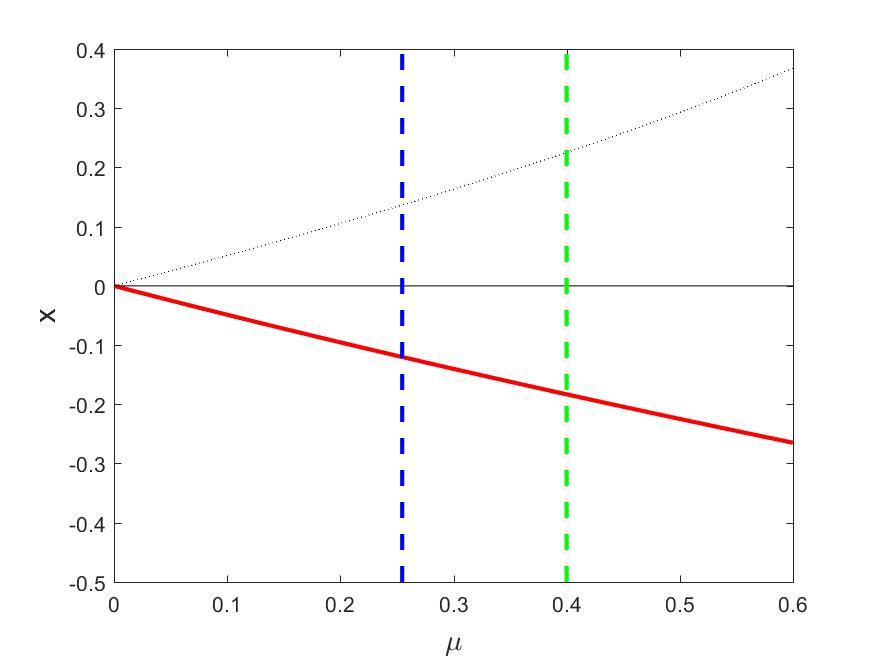
\includegraphics[width=.7\textwidth]{oneD/osc_cases.jpg}
\caption{The parameter ranges for each case is shown here with $A=2$. For reference, the original bifurcation diagram is overlayed.}
\label{fig:oneD_osc_cases}
\end{figure}

\subsection{Case I: $v_0(t) \le -|A|$}
\label{subsec:oneD_osc_CaseI}

We call this the entirely below axis case as the solution stays far from the axis $x=0$ for most of the oscillation and thus the behavior is not influenced by the non-smooth dynamics. We don't expect to see the bifurcation occur under these conditions but instead we find the parameter range for the cases. Here the integral in equation \eqref{eq:oneD_osc_integral} is straightforward to evaluate as $v_0(t)$ is a constant with respect to the 'fast' time $T$, thus we find the inner equation and equilibrium

\begin{equation*}
{v_0}_t=-m-2v_0,\quad v_0=-\frac{m}{2}.
\end{equation*}

This gives the leading order equilibrium solution with oscillations to our inner equation for this case which we write in the original variables

\begin{equation}\label{eq:oneD_osc_caseIsoln}
\begin{aligned}
y(t,T)\sim& -\frac{m}{2}-A\cos(T)+O(\Omega^{-1}),\\ 
x(t)\sim& -\frac{\mu}{2}-\Omega^{-1} A\cos(\Omega t)+O(\Omega^{-2}).
\end{aligned}
\end{equation}

The condition $v_0(t)\le -|A|$ combined with the equilibrium allows us to establish when \eqref{eq:oneD_osc_caseIsoln} holds

\begin{equation}\label{eq:oneD_osc_caseboundary}
\mu\ge \frac{2|A|}{\Omega}.
\end{equation}

Following the equilibrium to \eqref{eq:oneD_osc_caseboundary} leads us to Case II where the oscillations cross the axis and the assumptions of this case no longer hold.

\subsection{Case II: $|v_0(t)|< |A|$}
\label{subsec:oneD_osc_CaseII}

We call this the crossing case; here the equilibrium is small enough that the oscillations can now push the equilibrium above the axis. Under these conditions, the solution spends time near the axis $x=0$ and thus experiences the non-smooth influence. As the crossing continues, the non-smooth behavior drives the solution to gradually grow and thus we expect to find the bifurcation here. From \eqref{eq:oneD_osc_caseboundary}, we have a range of $\mu$ for when this case applies, $\mu<\frac{2|A|}{\Omega}$. But the integrand in \eqref{eq:oneD_osc_integral} is non-trivial when $|v_0(t)|<|A|$. In order to deal with the sign changing inside the integral, we break the integration into regions based on sign. Recall that we are searching for equilibrium behavior, and so we may make the assumption that we are dealing with a fixed value of $v_0$ such that $|v_0|\le |A|$. In figure~\ref{fig:oneD_osc_t1t2_graphic} we observe the function that we are integrating.

\begin{figure}[H]
\centering
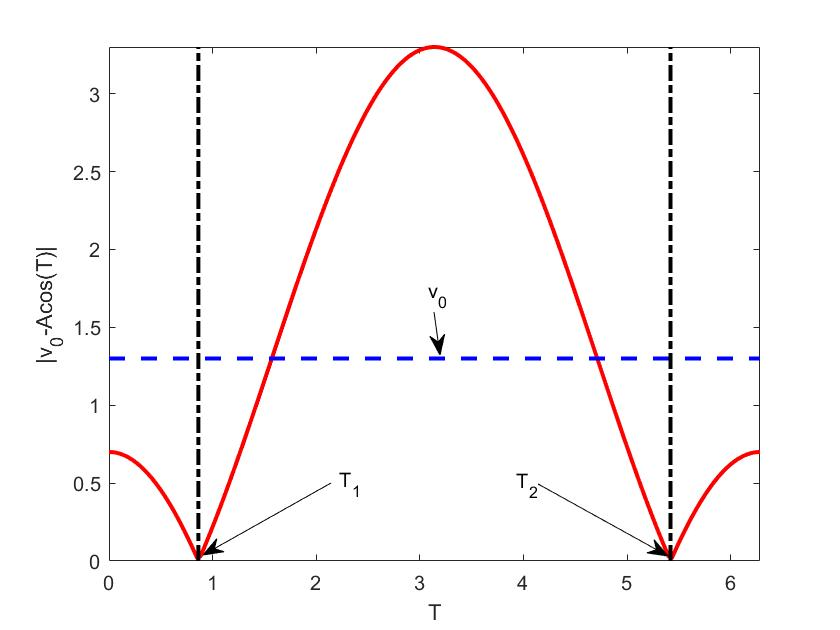
\includegraphics[width=0.7\textwidth]{oneD/t1t2_graphic.jpg}
\caption{The non-smooth function $|y_0|=|v_0-A\cos(T)|$ that we integrate is shown as the solid red line. We also show an example of $v_0$ as a horizontal blue dotted line. Here the value of $|v_0|\le|A|$, which causes kinks to appear at the roots of $|y_0|$, $T_1$ and $T_2$ respectively which are vertical black dashed dotted lines. }
\label{fig:oneD_osc_t1t2_graphic}
\end{figure}

We now consider the following roots of the integrand with 

\begin{equation*}
T_1=\arccos (v_0/A),\qquad T_2= 2\pi - \arccos (v_0/A).
\end{equation*}

Here we notice $0<T_1<T_2<2\pi$ and that the sign of the integrand stays the same on each interval. We only assume that the interval $[0,T_1]$ is following the solution while the center is still negative, thus the integrand will also be negative. From this, the integral is

\begin{equation}\label{eq:oneD_osc_expandedintegral}
\begin{aligned}
\int_0^{2\pi}|v_0-A\cos(T)|\,dT=&-\int_0^{T_1}(v_0-A\cos(T))\,dT+\\
&\int_{T_1}^{T_2}(v_0-A\cos(T))\,dT-\int_{T_2}^{2\pi}(v_0-A\cos(T))\,dT.
\end{aligned}
\end{equation}

Evaluating \eqref{eq:oneD_osc_expandedintegral} and using a trig identity, $\sin(\arccos(x))=\sqrt{1-x^2}$, we find the integral to be

\begin{equation*}
\int_0^{2\pi}|v_0-A\cos(T)|\,dT=\frac{2}{\pi}\left(\arcsin(v_0/A)v_0+\sqrt{A^2-v_0^2}\right).
\end{equation*}

Now, we notice that our argument above is simple for $v_0$ in equilibrium, but we have used a multiple scales approach for our 'fast' time with $t\ll T$ implying that $v_0(t)$ is approximately fixed over $T\in [0,2\pi]$. This holds true due to having a high frequency $\Omega$ and otherwise would not be a valid approximation. Thus we can evaluate \eqref{eq:oneD_osc_integral} to find the inner equation 

\begin{equation}\label{eq:oneD_osc_caseIIexact}
{v_0}_t=-m+\frac{4}{\pi}\left(\arcsin(v_0/A)v_0+\sqrt{A^2-v_0^2}\right).
\end{equation}

But in its current form, \eqref{eq:oneD_osc_caseIIexact} restricts any explicit form for $v_0(t)$, so we use a quadratic Taylor approximation to be able to solve this equation explicitly

\begin{equation}\label{eq:oneD_osc_caseIItaylor}
{v_0}_t \approx -m + \frac{4|A|}{\pi} + \frac{2}{\pi |A|}v_0^2,
\end{equation}

which has the following equilibrium with positive constant $C$

\begin{equation}\label{eq:oneD_osc_caseIIequil}
v_0=-C\sqrt{m-\frac{4|A|}{\pi}}.
\end{equation}

Thus we have the leading order inner equilibrium solution \eqref{eq:oneD_osc_caseIIequil} and we translate back into the original coordinates

\begin{equation}\label{eq:oneD_osc_innersoln}
\begin{aligned}
y\sim& -C\sqrt{m-\frac{4|A|}{\pi}}-A\cos(T)+O(\Omega^{-1}),\\ 
x(t)\sim& -C\sqrt{\Omega \left(\mu-\frac{4|A|}{\pi \Omega}\right)}-\Omega^{-1} A\cos(\Omega t)+O(\Omega^{-2}).
\end{aligned}
\end{equation}

It then is clear that the bifurcation, $\mu_{\text{osc}}$, occurs when \eqref{eq:oneD_osc_innersoln} fails to be real valued. Thus here we find $\mu_{\text{osc}}$ to take the form

\begin{equation}\label{eq:oneD_osc_bif}
\mu_{\text{osc}}=\frac{4|A|}{\pi \Omega}.
\end{equation}

From the result \eqref{eq:oneD_osc_bif}, we gather that the oscillatory forcing in the system causes the bifurcation to occur sooner and that this is controlled by the size of $A$ and $\Omega$. This should be expected as the model experiences the non-smooth behavior sooner in $\mu$ with the oscillations as opposed to later in $\mu$ with the slow variation. This effect is contrary to the slow variation where the solution experienced a delayed tipping whereas with oscillatory forcing the solution experiences a bifurcation $\mu_{\text{osc}}>\mu_{ns}$. This also indicates that the region of bi-stability is shrunk with oscillatory forcing and thus can be used to eliminate the region entirely with $A$ and $\Omega$ chosen properly, effectively destroying any hysteresis. We compare our estimate to numerical results for varying sizes of $\Omega^{-1}$.

\begin{figure}[H]
\centering
\begin{subfigure}{.5\textwidth}
 \centering
 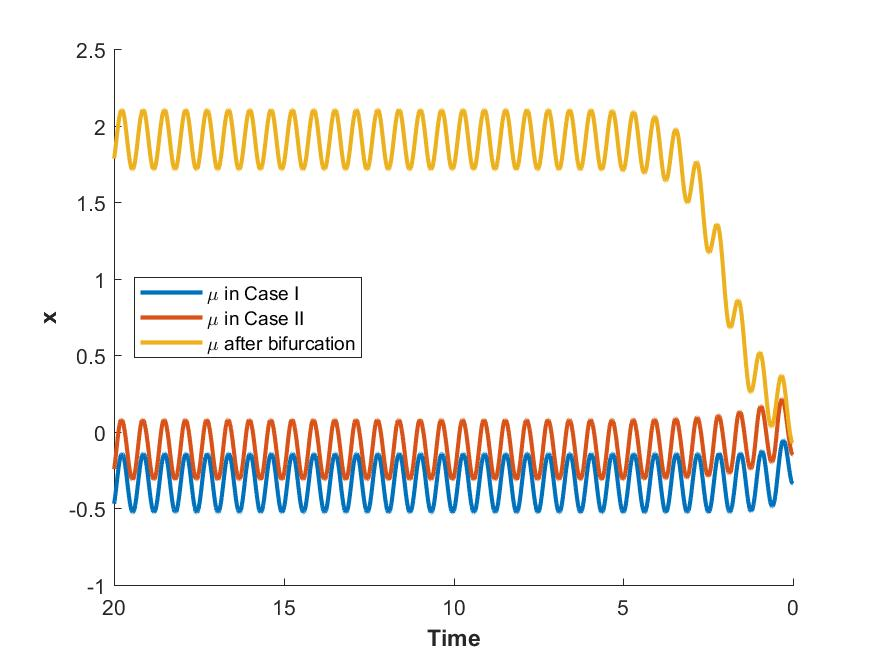
\includegraphics[width=\linewidth]{oneD/osc_timeseries.jpg}
 \caption{}
\end{subfigure}%
\begin{subfigure}{.5\textwidth}
 \centering
 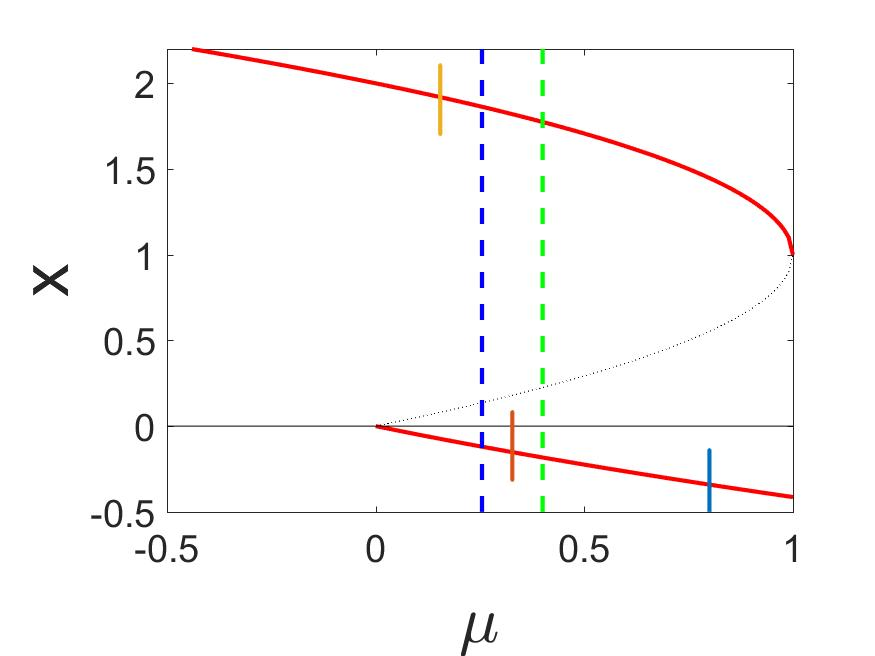
\includegraphics[width=\linewidth]{oneD/osc_bif_diagram.jpg}
 \caption{}
\end{subfigure}
\begin{subfigure}{.5\textwidth}
 \centering
 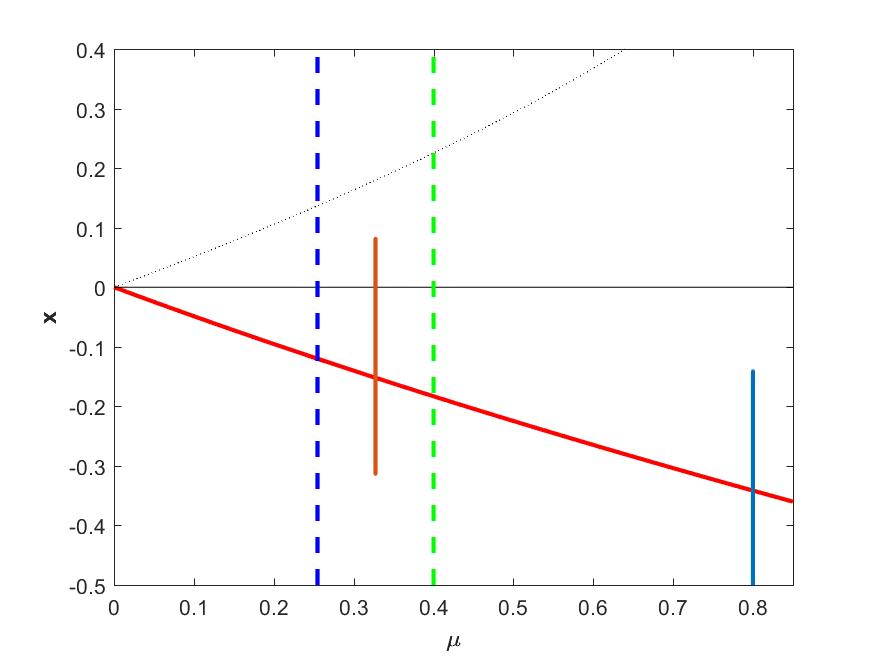
\includegraphics[width=\linewidth]{oneD/osc_bif_diagram_zoom.jpg}
 \caption{}
\end{subfigure}%
\begin{subfigure}{.5\textwidth}
\centering
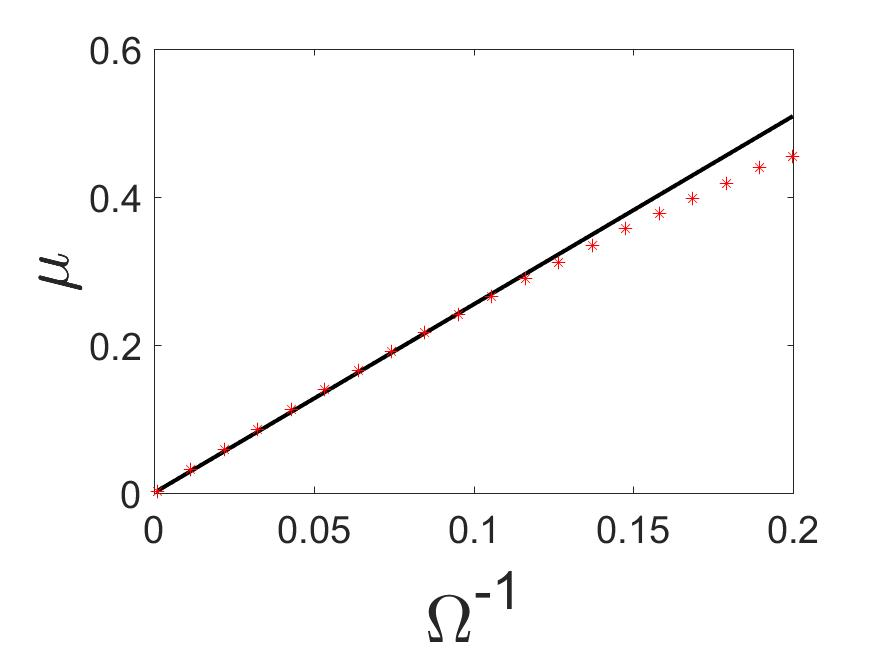
\includegraphics[width=\linewidth]{oneD/osc_Omegacomp.jpg}
\caption{}
\label{fig:oneD_osc_comp}
\end{subfigure}
\caption{In (a) the numerical time series solutions to \eqref{eq:oneD_canonical} are given from bottom to top with $\mu=\{.8,.33,.15\}$ in Case I, Case II and $\mu<\mu_{\text{osc}}$ in \eqref{eq:oneD_osc_bif} respectively with $A=2$, $\Omega=10$ and $\epsilon=0$. In (b) we show the time series on the bifurcation diagram. As shown by (c), a zoom in closer to the non-smooth bifurcation, where the dotted vertical lines dictate the region between Case I and Case II (green) as well as the bifurcation estimate (blue) respectively. In (d) a range of $\Omega^{-1}$ and their corresponding numerical bifurcations (red stars) are compared to our estimate of the bifurcation (black solid line). We consider the numeric bifurcation to be when the solution has passed $x>.5$.}
\label{fig:oneD_osc_numerics}
\end{figure}

In figure~\ref{fig:oneD_osc_numerics} an example is shown of the effect oscillatory forcing has given a choice of $A$ and $\Omega$ with (a), (b) and (c), but (d) shows the bifurcation approximation across a range of $\Omega^{-1}$. There is an allowed range of $\Omega$ from our assumption of $\Omega \gg 1$, which in this region we see agreement. The concavity is well represented and the behavior as $\Omega^{-1}\to 0$ converges to the standard bifurcation. Then we expect that our methodology is valuable for the Stommel problem.

\subsection{Stability}

Once more, we have that the outer solution \eqref{eq:oneD_osc_outersoln} is stable from the static model in \autoref{sec:oneD_static}. In this section, we have two regions of interest and establish their stabilities agree with our analysis. Each region has a particular version of the same inner equation dictating the solution's behavior

\begin{equation}\label{eq:oneD_osc_stabilityI}
{v_0}_t=-m+\frac{1}{\pi}\int_0^{2\pi}|v_0-A\cos(T)|\,dT.
\end{equation}

\subsubsection{Case I: $v_0(t)< -|A|$}

In this region we didn't find any bifurcating behavior and \eqref{eq:oneD_osc_stabilityI} simplifies and has the inner equation and equilibrium as follows

\begin{equation*}
{v_0}_t=-m-2v_0=f(v_0), \quad z^0=-\frac{m}{2}.
\end{equation*}

Similarly to \autoref{sec:oneD_slow}, we have a fixed parameter equation that we have shown to cause perturbations to decay exponentially and hence we find the equilibrium to be hyperbolic and asymptotically stable in the paramter range found in the analysis \eqref{eq:oneD_osc_caseboundary}

\begin{equation*}
\mu \ge \frac{2|A|}{\Omega}.
\end{equation*}

\subsubsection{Case II: $|v_0(t)|<|A|$}

For this region we found a bifurcation and the Taylor approximation \eqref{eq:oneD_osc_caseIItaylor} for the inner equation and equilibrium to be

\begin{equation}\label{eq:oneD_osc_stabilityII}
{v_0}_t= -m +\frac{4|A|}{\pi}+\frac{2}{\pi |A|}v_0^2,\quad z^0=-C \sqrt{m-\frac{4|A|}{\pi}}.
\end{equation}

We consider a simple linear perturbation of \eqref{eq:oneD_osc_stabilityII}, $v_0(t)=z^0+u(t)$ with $\lVert u(t) \rVert \ll 1$. Applying the standard Taylor expansion to determine the equation for the perturbations, we find

\begin{equation}\label{eq:oneD_osc_innerpertubation}
\begin{aligned}
{v_0}_t =& f(z^0)+f_{v_0}(z^0)(v_0-z^0)+ O(\lVert v_0-z^0\rVert^2),\\ 
u_t =& f(z^0)+f_{v_0}(z^0)u+O(\lVert u \rVert^2),\\
u_t =& -2\sqrt{m-\frac{4|A|}{\pi}} u .
\end{aligned}
\end{equation}

From \eqref{eq:oneD_osc_innerpertubation}, the sign gives that the perturbations decay exponentially and hence the equilibrium is hyperbolic and asymptotically stable as long as $m>\frac{4|A|}{\pi}$ or $\mu>\frac{4|A|}{\pi \Omega}$. We find that once $\mu$ reaches the value in \eqref{eq:oneD_osc_bif}, then the stability of \eqref{eq:oneD_osc_innerpertubation} is non-hyperbolic. When the stability switches like this, we expect a bifurcation, thus we have further evidence to support that \eqref{eq:oneD_osc_bif} is the oscillatory bifurcation we seek.

\section{Slowly Varying and Oscillatory Forcing}
\label{sec:oneD_slowosc}

Since we have established an approach for each feature of the problem individually, we combine them in the full one-dimensional model \eqref{eq:oneD_canonical} with $\epsilon\ll 1$ and ${A\sim O(1)}$. Once again, due to the slow variation in $\mu$, we do not see a bifurcation occur under these conditions but rather a tipping point. Hence we must find the behavior of the solution and search for when a rapid transition towards the upper branch occurs. We also seek a relationship between the slow drift and the high frequency, so we consider a generic polynomial $\Omega = \epsilon^{-\lambda}$ with parameter $\lambda>0$ relationship. With a general $\lambda$, we classify regions of behavior by ranges of $\lambda$ and have access to the boundaries of mixed behavior against one of the mechanisms becoming dominant. With both mechanisms in effect, we again choose to use a multiple scales approach that captures both slow behavior and fast oscillations. But now, we truly have 'slow' time, the slowly varying parameter $\mu(t)$, as well as 'fast' time, the rapid oscillations $\sin(\Omega t)$. The choice in time scales is then $\tau=\epsilon t$ and $T=\epsilon^{-\lambda} t$, which leads to the system

\begin{equation*}
\begin{aligned}
x_T+\epsilon^{\lambda+1}x_\tau =& \epsilon^\lambda (-\mu(\tau)+2|x|-x|x|+A\sin(T)),\\
\mu_\tau(\tau)=&-1.
\end{aligned}
\end{equation*}

Once again, we assume initial conditions in the region $x<0$ and start far enough out before any crossing occurs to find the outer solution. Thus we have the system

\begin{equation}\label{eq:oneD_slowosc_outereq}
\begin{aligned}
x_T+\epsilon^{\lambda+1}x_\tau =& \epsilon^\lambda (-\mu(\tau)-2x+x^2+A\sin(T)),\\
\mu_\tau(\tau)=&-1.
\end{aligned}
\end{equation}

We consider an asymptotic expansion in terms of the small quantity $\epsilon^\lambda$, where we note that this is the same as $\Omega^{-1}$,

\begin{equation}\label{eq:oneD_slowosc_asympexpansion}
x(\tau,T)\sim x_0(\tau,T)+\epsilon^\lambda x_1(\tau,T)+O(\epsilon^{1+\lambda},\epsilon^{2\lambda}).
\end{equation}

Introducing the expansion \eqref{eq:oneD_slowosc_asympexpansion} into the outer multi-scaled equation \eqref{eq:oneD_slowosc_outereq} gives 

\begin{equation}\label{eq:oneD_slowosc_outerexplicit}
{x_0}_T+\epsilon^{\lambda+1}{x_0}_\tau+\epsilon^\lambda {x_1}_T+\ldots=\epsilon^\lambda(-\mu(\tau)-2x_0+x_0^2+A\sin(T))+\epsilon^{2\lambda}(-2x_1+x_1x_0)+\ldots
\end{equation}

Here we separate \eqref{eq:oneD_slowosc_outerexplicit} to find the following system of equations from each order of $\epsilon^\lambda$

\begin{align}
\label{eq:oneD_slowosc_outerO1}
O(1):\quad & {x_0}_T=0, \\
\label{eq:oneD_slowosc_outerO2}
O(\epsilon^\lambda):\quad& {x_1}_T=-\mu(\tau)-2x_0+x_0^2+A\sin(T),\\
\label{eq:oneD_slowosc_outerO3}
O(\epsilon^{2\lambda}):\quad& {x_2}_T+\epsilon^{1-\lambda}{x_0}_\tau= -2x_1+2x_0x_1.
\end{align}

Depending on the value of $\lambda$, $O(\epsilon^{\lambda+1})$ may be the next order before $O(\epsilon^{2\lambda})$, although considering either produce the same equation at their respective order and hence our choice in $\lambda$ doesn't change the calculations up to this correction term. Thus for the outer solution, we consider the system with $O(\epsilon^{2\lambda})$. Each equation gives the behavior of each order of the solution; \eqref{eq:oneD_slowosc_outerO1} indicates that the leading order term is purely slow dependent, $x_0=x_0(\tau)$. In \autoref{app:oneD} we apply the Fredholm alternative \eqref{eq:Fredholm} to \eqref{eq:oneD_slowosc_outerO2} and \eqref{eq:oneD_slowosc_outerO3} to find the first few terms of the expansion in \eqref{eq:oneD_slowosc_asympexpansion} explicitly. The resulting solution is

\begin{equation}\label{eq:oneD_slowosc_outersoln}
x\sim 1-\sqrt{1+\mu(t)}-\frac{\epsilon}{4(1+\mu(t))}-\epsilon^\lambda A \cos(\Omega t)+O(\epsilon^{1+\lambda},\epsilon^{2\lambda}).
\end{equation}

In the outer solution \eqref{eq:oneD_slowosc_outersoln}, we consider when the terms violate the assumptions of the expansion to find where we need to use an inner equation. This happens either when $x_0\sim O(\epsilon)$ or when $x_0\sim O(\epsilon^\lambda)$ where we suspect is when $\mu\sim O(\epsilon)$ or $\mu\sim O(\epsilon^\lambda)$ respectively, the occurrence of which depends on $\lambda$. 

To find an inner equation we use a general scaling for both $x$ and $\mu$ given the ambiguity of choice in $\mu$ with

\begin{equation}\label{eq:oneD_slowosc_general_scaling}
x=\epsilon^\alpha y ,\quad \mu(t)=\epsilon^\beta m(t),
\end{equation}

where we anticipate $\alpha>0$ and $\beta>0$. Applying the scaling \eqref{eq:oneD_slowosc_general_scaling} to the canonical equation \eqref{eq:oneD_canonical} gives

\begin{equation}\label{eq:oneD_slowosc_innerscaled}
\begin{aligned}
\epsilon^\alpha \dot{y}=& -\epsilon^\beta m(t)+\epsilon^\alpha 2|y| - \epsilon^{2\alpha}y|y| +A\sin(\epsilon^{-\lambda}t),\\
\dot{m}(t)=&-\epsilon^{1-\beta}.
\end{aligned}
\end{equation}

From \eqref{eq:oneD_slowosc_innerscaled} we find the 'fast' time still appears but the 'slow' time has multiple choices depending on $\lambda$. For convenience we choose to take a multiple scales approach with scales $t$ and $T=\epsilon^{-\lambda}t$ in \eqref{eq:oneD_slowosc_innerscaled} to find

\begin{equation}\label{eq:oneD_slowosc_innergeneral}
\begin{aligned}
\epsilon^{\alpha-\lambda} y_T+\epsilon^{\alpha}y_t=& -\epsilon^{\beta}m(t)+\epsilon^{\alpha}2|y|-\epsilon^{2\alpha}y|y|+A\sin(T),\\
m_t(t)=&-\epsilon^{1-\beta}.
\end{aligned}
\end{equation}

To determine the correct scalings in \eqref{eq:oneD_slowosc_general_scaling}, we balance the leading order terms on both sides of \eqref{eq:oneD_slowosc_innergeneral} $\epsilon^{\alpha-\lambda}y_T$ and $A\sin(T)$, which gives us that $\alpha=\lambda$. This suggests the oscillatory term persists in the inner asymptotic expansion of \eqref{eq:oneD_canonical} regardless of choice in $\lambda$.

We now consider the same scales $t$ and $T=\epsilon^{-\lambda}t$ on the canonical system \eqref{eq:oneD_canonical} 

\begin{equation}\label{eq:oneD_slowosc_general_outermulti}
\begin{aligned}
x_T+\epsilon^{\lambda}x_t =& -\epsilon^{\lambda+\beta}m(t)+\epsilon^{\lambda}2|x|-\epsilon^{\lambda}x|x|+\epsilon^{\lambda}A\sin(T),\\
m_t(t) =&-\epsilon^{1-\beta}.
\end{aligned}
\end{equation}

Here we use the expansion 

\begin{equation*}
x(t,T) = \epsilon^{\lambda}y_0(t,T) +\ldots 
\end{equation*}

where the next terms of this expansion depend on whether $\lambda\le1$ or if $\lambda> 1$. We consider these ranges as Case I and Case II respectively.

\subsection{Case I: $\lambda \le 1$}
\label{subsec:oneD_slowosc_caseI}

We call this the mixed effects case due to both slow variation and oscillatory forcing causing noticeable effects on the solution for this range of $\lambda$. We consider the expansion

\begin{equation}\label{eq:oneD_slowosc_caseI_expansion}
x(t,T)\sim \epsilon^{\lambda} y_0(t,T)+\epsilon^q y_1(t,T)+\ldots
\end{equation}

with $q>\lambda$ to be consistent with the scale analysis above that determined inner behavior to start at $O(\epsilon^\lambda)$. Substituting \eqref{eq:oneD_slowosc_caseI_expansion} into \eqref{eq:oneD_slowosc_general_outermulti} gives

\begin{equation*}
\begin{aligned}
{y_0}_T+\epsilon^{\lambda}{y_0}_t+\epsilon^{q-\lambda} {y_1}_T+\epsilon^{q} {y_1}_t+\ldots={} & -\epsilon^{\beta}m(t)+\epsilon^\lambda 2|y_0 +\epsilon^{q-\lambda} y_1+\ldots|+ A\sin(T) \\
& + \epsilon^{2\lambda}( y_0 +\epsilon^{q-\lambda} y_1+\ldots)|y_0 +\epsilon^{q-\lambda} y_1+\ldots |
\end{aligned}
\end{equation*}

Separation by distinct orders of $\epsilon$ then gives the following equations at each order

\begin{align} \label{eq:oneD_slowosc_caseI_O1}
O(1):\, & {y_0}_T = A\sin(T),\\ \label{eq:oneD_slowosc_caseI_O2}
O(\epsilon^\lambda): \, & \epsilon^{q-2\lambda}{y_1}_T+{y_0}_t=-\epsilon^{\beta-\lambda}m(s)+2|y_0|.
\end{align}

In \eqref{eq:oneD_slowosc_caseI_O2} we find the appropriate next term in the expansion \eqref{eq:oneD_slowosc_caseI_expansion} is with $q=2\lambda$. This choice in $q$ keeps the equations balanced but $q$ implies that $\lambda> \frac{1}{2}$ for an expansion to be found. Otherwise, the quadratic terms must be included and we no longer find local equations. This indicated that the range of $\lambda\le\frac{1}{2}$ behaves differently and we discuss this further in \autoref{chap:conclusion}. We also have the choice between $\beta=\lambda$ or $\beta=1$ and each has a particular appeal. With $\beta=\lambda$, the form of \eqref{eq:oneD_slowosc_caseI_O2} is simple, but the equation for the slow variation is $m_t=-\epsilon^{1-\lambda}$. The slow variation equation suggests slower time scale to approach the problem. We instead choose to allow $\beta=1$ for convenience and track the small coefficient on $m(t)$ now in exchange for staying on the same time scale with $m_t=-1$. This is valid as long as we are tracking small coefficients and not large ones, as this would suggest we used an incorrect scaling, but both of these choices lead to the same conclusion. Using \eqref{eq:oneD_slowosc_caseI_O1} gives the appropriate separation in slow and fast scales, $y_0(t,T)=v_0(t)-A\cos(T)$. We then apply the Fredholm alternative \eqref{eq:Fredholm} to \eqref{eq:oneD_slowosc_caseI_O2} which gives a similar equation to the integral \eqref{eq:oneD_osc_integral} in \autoref{sec:oneD_highfreqosc} with

\begin{equation}\label{eq:oneD_slowosc_caseIintegral}
{v_0}_t = -\epsilon^{1-\lambda}m(t)+\frac{1}{\pi}\int_0^{2\pi} |v_0(t)-A\cos(T)|\,dT.
\end{equation}

The approach developed in \autoref{sec:oneD_highfreqosc} is applied here to \eqref{eq:oneD_slowosc_caseIintegral}, where we separate the behavior of the integral based on the relative size of $v_0(t)$ to $A$. We have the following situations, Sub-Case I: $v_0(t)\le -|A|$ and Sub-Case II: $|v_0(t)|<|A|$.

\subsubsection{Sub-Case I: $v_0(t) \le -|A|$} 
\label{subsubsec:oneD_slowosc_subcaseI}

Once more, we call this the entirely below axis sub-case, here we don't expect tipping to occur under these conditions since the solution is entirely negative and far from the axis $x=0$ for most of the oscillation. Under these conditions, \eqref{eq:oneD_slowosc_caseIintegral} gives the simple inner equation

\begin{equation}\label{eq:oneD_slowosc_innersubcaseI}
{v_0}_t= -\epsilon^{1-\lambda}m(t)-2v_0.
\end{equation}

Solving \eqref{eq:oneD_slowosc_innersubcaseI} can be done under our assumptions much like in \autoref{subsec:oneD_osc_CaseI} but instead we focus on the pseudo-equilibrium. This choice results in finding the effective parameter range for $\mu$ which distinguishes these sub-cases, which helps to determine when the solution enters the parameter range for Sub-Case II. Since $m(t)$ is allowed to vary, this must be thought of more as a pseudo-equilibrium and we are only interested in when the pseudo-equilibrium violates the assumptions of this case. Finding the pseudo-equilibrium of \eqref{eq:oneD_slowosc_innersubcaseI} gives

\begin{equation*}
v_0(t)=-\epsilon^{1-\lambda}\frac{m(t)}{2}.
\end{equation*}

Using the condition $v_0(t)\le -|A|$ gives that $m(t)\ge \epsilon^{\lambda-1}2|A|$. Writing this result in original coordinates gives us the parameter range for Sub-Case I

\begin{equation}\label{eq:oneD_slowosc_subcaseboundary}
\mu(t)\ge \frac{2 |A|}{\Omega},
\end{equation}

which agrees with the range from \eqref{eq:oneD_osc_caseboundary} in \autoref{sec:oneD_highfreqosc}. Following the pseudo-equilibrium to the boundary \eqref{eq:oneD_slowosc_subcaseboundary}, we eventually reach Sub-Case II where we see the oscillations crossing the axis.

\subsubsection{Sub-Case II: $|v_0(t)|< |A|$}
\label{subsubsec:oneD_slowosc_subcaseII}

Again, we call this the crossing sub-case. Here the behavior of the solution depends strongly on the sign of the solution similarly to \autoref{sec:oneD_highfreqosc}, but we seek the relationship between slow variation and oscillatory forcing on the tipping point. As the pseudo-equilibrium get closer to the $x=0$ axis, the solution spends more time above this axis and more complicated contributions from the sign chinging appears. With this behavior, we expect tipping to happen under these conditions.

The methodology of solving the integral in \eqref{eq:oneD_slowosc_caseIintegral} holds identically to that of \autoref{subsec:oneD_osc_CaseII}. Here, we have a 'slow' time function $v_0(t)$ that is approximately fixed with respects to the 'fast' time $T$ under the multiple scales approach. Thus we evaluate by separating the sign of the integrand with the values $T_1=\arccos(v_0/A)$ and $T_2 = 2\pi-\arccos(v_0/A)$ to find

\begin{equation}\label{eq:oneD_slowosc_subcaseIIexact}
{v_0}_t=-\epsilon^{1-\lambda}m(t)+\frac{4}{\pi}\left(\arcsin(v_0/A)v_0+\sqrt{A^2-v_0^2}\right).
\end{equation}

We then chose to find an explicit analytic expression by approximating \eqref{eq:oneD_slowosc_subcaseIIexact} with a quadratic Taylor expansion. This gives

\begin{equation}\label{eq:oneD_slowosc_subcaseIItaylor}
\begin{aligned}
{v_0}_t =& -\epsilon^{1-\lambda}m(t) + \frac{4|A|}{\pi} + \frac{2}{\pi |A|}v_0^2,\\
m_t =& -1.
\end{aligned}
\end{equation}

But as \eqref{eq:oneD_slowosc_subcaseIItaylor} is in terms of 'slow' time, it restricts any analytical approaches to the effects of the varying parameter. Instead we take the same approach from \cite{haberman1979slowly} and switch the differentiation onto the parameter $m$ with

\begin{equation}\label{eq:oneD_slowosc_subcaseIItaylorm}
{v_0}_m = \epsilon^{1-\lambda}m - \frac{4|A|}{\pi} - \frac{2}{\pi |A|}v_0^2.
\end{equation}

It is here we take advantage of the form of \eqref{eq:oneD_slowosc_subcaseIItaylorm} with the form from Zhu \& Kuske \eqref{eq:intro_Zhuairy} to solve which results in

\begin{equation*}
v_0(m)\sim \epsilon^{(1-\lambda)/3}\left( \frac{\pi |A|}{2} \right)^{2/3}\frac{Ai'\left(\epsilon^{2(\lambda-1)/3}\left(\frac{2}{\pi |A|}\right)^{1/3}(\epsilon^{1-\lambda}m-\frac{4|A|}{\pi})\right)}{Ai\left(\epsilon^{2(\lambda-1)/3}\left(\frac{2}{\pi |A|}\right)^{1/3}(\epsilon^{1-\lambda}m-\frac{4|A|}{\pi})\right)}.
\end{equation*}

With the solution to \eqref{eq:oneD_slowosc_caseI_expansion} we rewrite back into the original coordinates

\begin{equation}\label{eq:oneD_slowosc_caseIsoln}
\begin{aligned}
y_0(t,T)\sim& C\frac{Ai'\left(\epsilon^{2(\lambda-1)/3}\left(\frac{2}{\pi |A|}\right)^{1/3}(\epsilon^{1-\lambda}m(t)-\frac{4|A|}{\pi})\right)}{Ai\left(\epsilon^{2(\lambda-1)/3}\left(\frac{2}{\pi |A|}\right)^{1/3}(m(t)-\frac{4|A|}{\pi})\right)}-\epsilon^\lambda A\cos(T)+\ldots,\\
x(t) \sim& C\frac{Ai'\left(\left(\frac{\Omega}{\epsilon^2}\right)^{1/3}\left(\frac{2}{\pi |A|}\right)^{1/3}(\mu(t)-\frac{4|A|}{\pi \Omega})\right)}{Ai\left(\left(\frac{\Omega}{\epsilon^2}\right)^{1/3}\left(\frac{2}{\pi |A|}\right)^{1/3}(\mu(t)-\frac{4|A|}{\pi \Omega})\right)}-\epsilon^\lambda A\cos(\Omega t) +\ldots.
\end{aligned}
\end{equation}

With the inner solution \eqref{eq:oneD_slowosc_caseIsoln} we search for the singularity of this solution in order to identify tipping. Recall from \eqref{eq:intro_Zhuresult} that the singularity relates to the first root of the Airy equation, which is when the argument is $-2.33811\ldots$. We find the singularity to be

\begin{equation}\label{eq:oneD_slowosc_uglymu}
\mu_{\text{mixed}}=\left(\frac{\epsilon^2}{\Omega}\right)^{1/3}\left(\frac{\pi |A|}{2}\right)^{1/3}(-2.33811\ldots)+\frac{4|A|}{\pi \Omega}.
\end{equation}

This value of $\mu$ that causes this singularity in turn is our tipping point, where we rewrite \eqref{eq:oneD_slowosc_uglymu} to show the contributions from slow variation of the parameter and the oscillatory forcing

\begin{equation}\label{eq:oneD_slowosc_caseItipping}
\mu_{\text{mixed}} = \left(\frac{1}{\epsilon\Omega}\right)^{1/3}\left(\frac{\pi |A|}{2}\right)^{1/3} \mu_{\text{smooth}}+\mu_{\text{osc}},
\end{equation}

with $\mu_{\text{smooth}}=\epsilon\left(-2.33811\ldots\right)$, similarly to the smooth problem from \cite{zhu2015tipping}, and $\mu_{\text{osc}}$ from \eqref{eq:oneD_osc_bif} respectively.

The resulting tipping approximation \eqref{eq:oneD_slowosc_caseItipping} indicates that the size of the amplitude $A$ determines whether the tipping occurs early or late relative to the bifurcation, naturally we see a larger amplitude cause more contribution from the oscillations and hence an earlier tipping. On the other hand, larger values in $\epsilon$ cause this tipping to occur later. So these effects have opposite pulls on the tipping and can effectively cancel one another out under the proper conditions. It would even be possible to break the hysteresis cycle by eliminating the region of bi-stability of this problem with sufficiently large amplitude and small $\epsilon$. This tipping holds for any $\lambda\in (\frac{1}{2},1]$ and we see different behavior for larger $\lambda$.

\subsection{Case II: $\lambda>1$}
\label{subsec:oneD_slowosc_caseII}

We call this the slow dominant case as this is when we see that the oscillations contribute less than the slow variation. For this range of $\lambda$ the scaling for $\mu$ is simple, $\mu=\epsilon m$ and thus we expect to see integer powers along with $\lambda$ powers so we choose the expansion

\begin{equation}\label{eq:oneD_slowosc_caseII_expansion}
x(t,T) \sim \epsilon^\lambda y_0(t,T)+\epsilon y_1(t,T)+\epsilon^q y_2(t,T)+\ldots
\end{equation}


where $q>\lambda$ to allow for consistency with the scale analysis but not necessarily the same value as in Case I. Substituting \eqref{eq:oneD_slowosc_caseII_expansion} into \eqref{eq:oneD_slowosc_general_outermulti} gives

\begin{equation*}
\begin{aligned}
\epsilon {y_0}_T+\epsilon^{\lambda+1} {y_0}_t+\epsilon^\lambda {y_1}_T+\epsilon^q {y_2}_T+\ldots=&-\epsilon^{\lambda+1}m(t)+\epsilon^{\lambda+1} 2|y_0+\epsilon^{\lambda-1} y_1 +\ldots|\\
&+ \epsilon^{\lambda+2}( y_0+\epsilon^{\lambda-1} y_1 +\ldots)| y_0+\epsilon^{\lambda-1} y_1 +\ldots|\\
&+\epsilon^\lambda A\sin(T) 
\end{aligned}
\end{equation*}

Here we separate out each order of $\epsilon$ to find the equations at each order

\begin{align} \label{eq:oneD_slowosc_caseII_O1}
O(\epsilon):\, &{y_0}_T=0,\\ \label{eq:oneD_slowosc_caseII_O2}
O(\epsilon^\lambda): \, & {y_1}_T = A\sin(T),\\ \label{eq:oneD_slowosc_caseII_O3}
O(\epsilon^{\lambda+1}):\, & \epsilon^{q-\lambda-1}{y_2}_T+ {y_0}_t = -m(t) +2|y_0+\epsilon^{\lambda-1}y_1|.
\end{align}

We learn in \eqref{eq:oneD_slowosc_caseII_O3} that $q=\lambda+1$ to keep terms from becoming trivial or unbalanced. From \eqref{eq:oneD_slowosc_caseII_O1} we find that the dominant behavior for this case is purely slow, $y_0=y_0(t)$. We find the oscillatory behavior in $y_1$ with \eqref{eq:oneD_slowosc_caseII_O2} which gives $y_1(t,T)=v_1(t)-A\cos(T)$. But as we have $y_1$ as a correction to $y_0$, we may absorb the slow behavior into $y_0$. Thus we treat $y_0(t)=y_0(t)+\epsilon^{\lambda+1} v_1(t)\approx y_0(t)$. Applying Fredholm to \eqref{eq:oneD_slowosc_caseII_O3} gives 

\begin{equation}\label{eq:oneD_slowosc_caseII_integral}
\begin{aligned}
{y_0}_t=& -m(t)+\frac{1}{\pi}\int_0^{2\pi}|y_0(t)-\epsilon^{\lambda-1}A\cos(T)|\,dT.
\end{aligned}
\end{equation}

With $\lambda$ being approximately 1, we see nearly identical behavior in \eqref{eq:oneD_slowosc_caseII_integral} as that of what we explored in \autoref{subsec:oneD_slowosc_caseI} as long as the amplitude of oscillations inside the integral are $\epsilon^{\lambda-1}A\sim O(1)$, then this integral is similar to the integral in Case I \eqref{eq:oneD_slowosc_caseIintegral}. To see this, we follow the same approach as to integrate \eqref{eq:oneD_slowosc_caseII_integral} with $T_1=\arccos(y_0/\epsilon^{\lambda-1}A)$ and $T_2=2\pi- \arccos(y_0/\epsilon^{\lambda-1}A)$ which gives

\begin{equation}\label{eq:oneD_slowosc_caseIIexact}
{y_0}_t=-m(t)+\frac{4}{\pi}\left(\arcsin(y_0/\epsilon^{\lambda-1}A)y_0+\sqrt{(\epsilon^{\lambda-1}A)^2-y_0^2}\right).
\end{equation}

Here we apply the same quadratic Taylor approximation to \eqref{eq:oneD_slowosc_caseIIexact} to find

\begin{equation}\label{eq:oneD_slowosc_caseII_taylor}
\begin{aligned}
{y_0}_t=&-m(t)+\epsilon^{\lambda-1}\frac{2|A|}{\pi}+\epsilon^{1-\lambda}\frac{2}{\pi |A|}y_0^2,\\
m=&-1.
\end{aligned}
\end{equation}

We use the result from Zhu \& Kuske \eqref{eq:intro_Zhuresult} to find the tipping, which we then write into original coordinates

\begin{equation*}
\begin{aligned}
m_{\text{mixed}}=&\epsilon^{(\lambda-1)/3}\left(\frac{\pi |A|}{2}\right)^{1/3}(-2.33811\ldots)+\epsilon^{\lambda-1}\frac{4|A|}{\pi},\\
\mu_{\text{mixed}}=&\left(\frac{1}{\epsilon\Omega}\right)^{1/3}\left(\frac{\pi |A|}{2}\right)^{1/3} \mu_{\text{smooth}}+\mu_{\text{osc}}.
\end{aligned}
\end{equation*}

We conclude that there is a natural transition into Case II from Case I with almost the same behavior and identical tipping as in \eqref{eq:oneD_slowosc_caseItipping}. As $\lambda$ continues to grow, the amplitude of oscillation in \eqref{eq:oneD_slowosc_caseII_integral} decays to . This allows us to say that the integral is approaching

\begin{equation}\label{eq:oneD_slowosc_caseII_inner}
{y_0}_t = -m(t) +2|y_0|.
\end{equation}

But \eqref{eq:oneD_slowosc_caseII_inner} has the same form as in \autoref{sec:oneD_slow} allowing us to use the results there to find the solution, where we put this back in terms of the original coordinates

\begin{equation}\label{eq:oneD_slowosc_caseIIsoln}
\begin{aligned}
y_0(t,T)\sim& C e^{-2m(t)}+\frac{m(t)}{2}-1/4 +\epsilon^\lambda A\cos(T),\\
x(t)\sim& C e^{-2\mu(t)/\epsilon}+\frac{\mu(t)}{2} -\epsilon^\lambda A\cos(\Omega t)+O(\epsilon^{2\lambda}).
\end{aligned}
\end{equation}

This then leads to the same tipping from the slow case with 

\begin{equation*}
\mu_{\text{slow}}=\frac{1}{2}\epsilon\log\epsilon.
\end{equation*}

Thus we find that in this case that for $\lambda$ near 1, the same $\mu_{\text{mixed}}$ tipping as in \eqref{eq:oneD_slowosc_caseItipping} occurs from \autoref{subsec:oneD_slowosc_caseI}. But for large $\lambda$, the oscillations have less of an impact and the solution tips entirely like $\mu_{\text{slow}}$ as in \eqref{eq:oneD_slow_tipping} from \autoref{sec:oneD_slow}. For convenience, this is summarized in the following table.

\begin{center}
\begin{table}[H]\label{table:oneD_tipping}
\centering
\begin{tabular}{|c|c|}
\hline 
 \multicolumn{2}{|c|}{One-Dimensional Tipping} \\ 
\hline
$\epsilon>0$ and $A=0$ & $\mu_{\text{slow}}=\epsilon\ln(\epsilon)/2$ \\ 
\hline 
$\epsilon=0$ and $A\not=0$ with $\Omega\gg1$ & $\mu_{\text{osc}}=\frac{4|A|}{\pi \Omega}$\\ 
\hline 
$\epsilon>0$, $A\not=0$ and $\lambda\le 1$: & $\mu_{\text{mixed}}=\epsilon^{(\lambda-1)/3}\left(\frac{\pi |A|}{2}\right)^{1/3} \mu_{smooth}+\mu_{osc}$ \\ 
\hline 
$\epsilon>0$, $A\not=0$ and $\lambda> 1$ with $\lambda\approx 1$: & $\mu_{\text{mixed}}=\epsilon^{(\lambda-1)/3}\left(\frac{\pi |A|}{2}\right)^{1/3} \mu_{smooth}+\mu_{osc}$ \\
\hline
$\epsilon>0$, $A\not=0$ and $\lambda>1$: & $ \mu_{\text{slow}}=\epsilon\ln(\epsilon)/2$\\
\hline
\end{tabular} 
\caption{The tipping of the one-dimensional model for each mechanism and case.}
\end{table}
\end{center}

In figure~\ref{fig:oneD_slowosc_numerical_small}, we see an example of the numerical solution to the canonical system \eqref{eq:oneD_canonical} with slow variation and oscillatory forcing. This example has tipping occurring in Case I due to $\lambda\in (\frac{1}{2},1]$ allowing the slow variation and oscillatory forcing to produce a mixed effect on the tipping. Although we see noticeable contributions from the slow varying parameter the tipping still is occurring in the region near the oscillatory bifurcation. This tells us that for these choices in the values the strongest effect is the oscillatory forcing. It is possible to find values of $\epsilon$, $A$ and $\lambda$ that cause the non-smooth tipping to occur at the same place as the smooth bifurcation. This in theory, would eliminate the region of bi-stability and destroy the hysteresis curve entirely for this model.

\begin{figure}[H]
\centering
\begin{subfigure}{.5\textwidth}
 \centering
 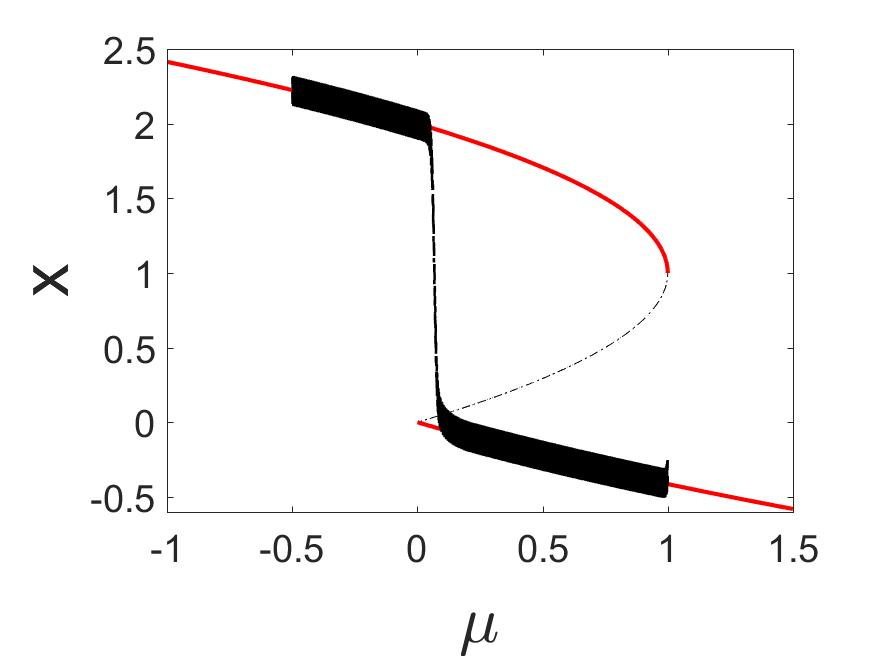
\includegraphics[width=\linewidth]{oneD/slowosc_bif_diagram_small.jpg}
 \caption{}
\end{subfigure}%
\begin{subfigure}{.5\textwidth}
 \centering
 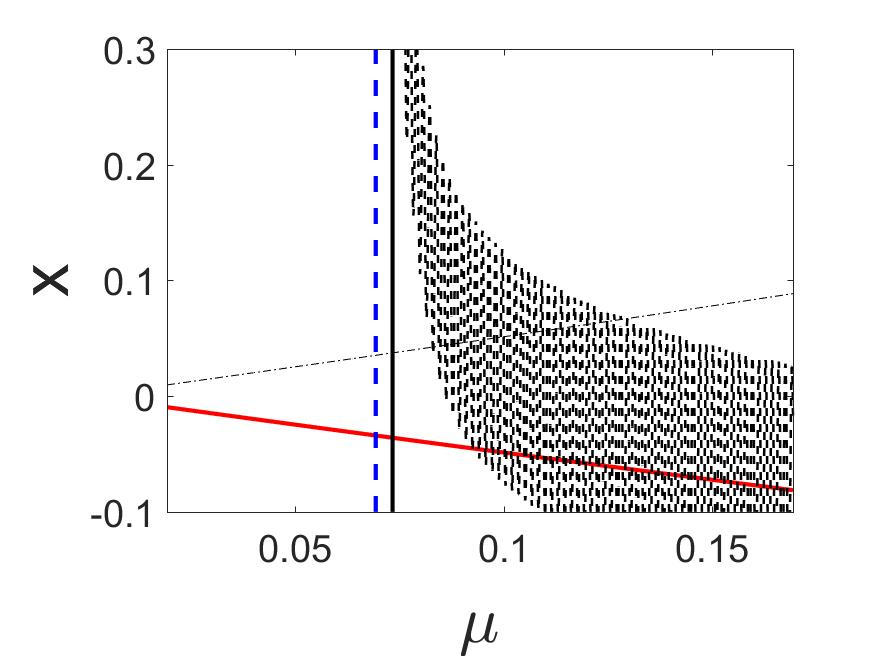
\includegraphics[width=\linewidth]{oneD/slowosc_bif_diagram_small_zoom.jpg}
 \caption{}
\end{subfigure}
\caption{Parameter values are $\epsilon=.05$, $\lambda=.8$ and $A=4$. On the left, this is the bifurcation diagram for the 1D system with the numerical solution to \eqref{eq:oneD_canonical} (black dotted line). On the right, this is a zoom in. The dotted vertical line is the tipping point $\mu_{\text{mixed}}$ \eqref{eq:oneD_slowosc_uglymu} (blue). The vertical line (black) is the numerically obtained tipping for $x>.5$.}
\label{fig:oneD_slowosc_numerical_small}
\end{figure}

In figure~\ref{fig:oneD_slowosc_numerical_medium}, we see an example of $\lambda$ falling into Case II but is close enough to 1 that we see mixed behavior in the tipping. Here the slow variation is now dominant and the oscillations are only noticeable in the zoom in. But the green dotted line is the tipping approximation \eqref{eq:oneD_slow_tipping} from \autoref{sec:oneD_slow}, and it doing better to approximation than the mixed tipping point.

\begin{figure}[H]
\centering
\begin{subfigure}{.5\textwidth}
 \centering
 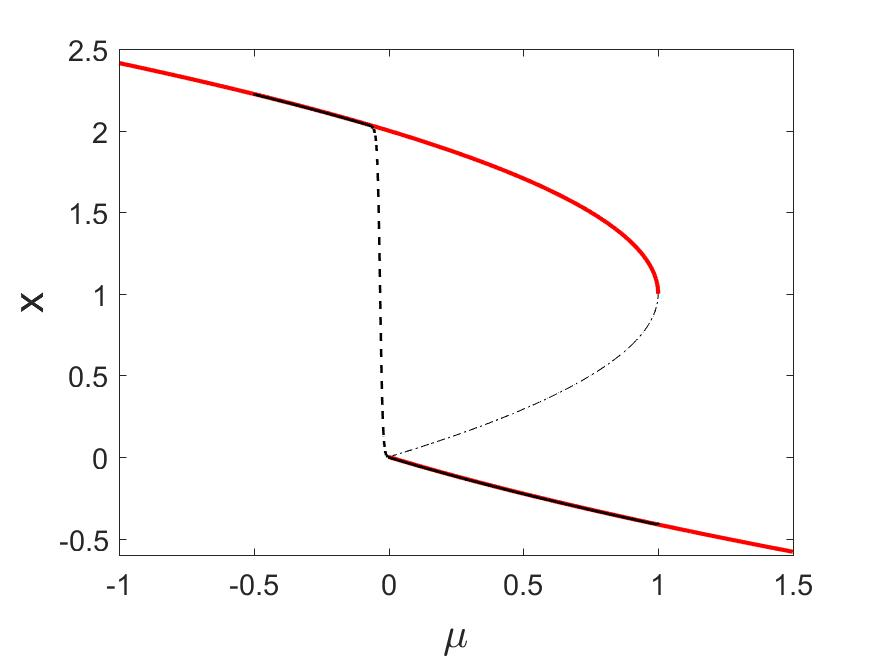
\includegraphics[width=\linewidth]{oneD/slowosc_bif_diagram_medium.jpg}
 \caption{}
\end{subfigure}%
\begin{subfigure}{.5\textwidth}
 \centering
 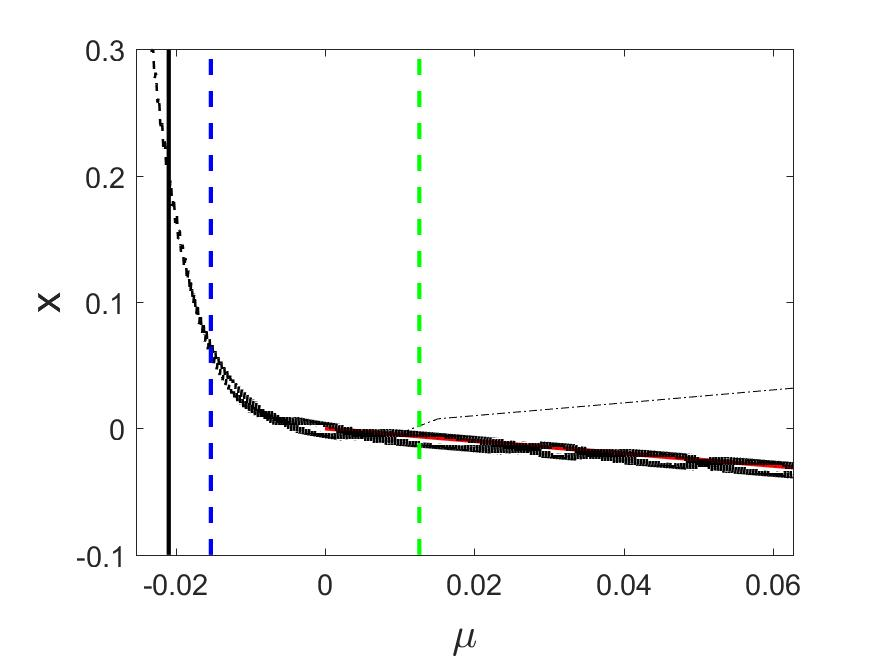
\includegraphics[width=\linewidth]{oneD/slowosc_bif_diagram_medium_zoom.jpg}
 \caption{}
\end{subfigure}
\caption{Parameter values are $\epsilon=.05$, $\lambda=1.05$ and $A=4$. On the left, this is the bifurcation diagram for the 1D system with the numerical solution to \eqref{eq:oneD_canonical} (black dotted line). On the right, this is a zoom in. The dotted vertical lines are the tipping point $\mu_{\text{mixed}}$ \eqref{eq:oneD_slowosc_uglymu} (blue) and slowly varying tipping $\mu_{\text{slow}}$ \eqref{eq:oneD_slow_tipping} (green). The vertical line (black) is the numerically obtained tipping for $x>.5$.}
\label{fig:oneD_slowosc_numerical_medium}
\end{figure}

In figure~\ref{fig:oneD_slowosc_numerical_large}, we see an example of $\lambda$ falling into Case II but is far enough from 1 that we see almost entirely slow behavior in the tipping. Even upon closer inspection there its hardly noticeable that oscillations are present in the model. The green dotted line is the tipping approximation \eqref{eq:oneD_slow_tipping} from \autoref{sec:oneD_slow}, and it is clear that this is a better approximation than the mixed tipping point.

\begin{figure}[H]
\centering
\begin{subfigure}{.5\textwidth}
 \centering
 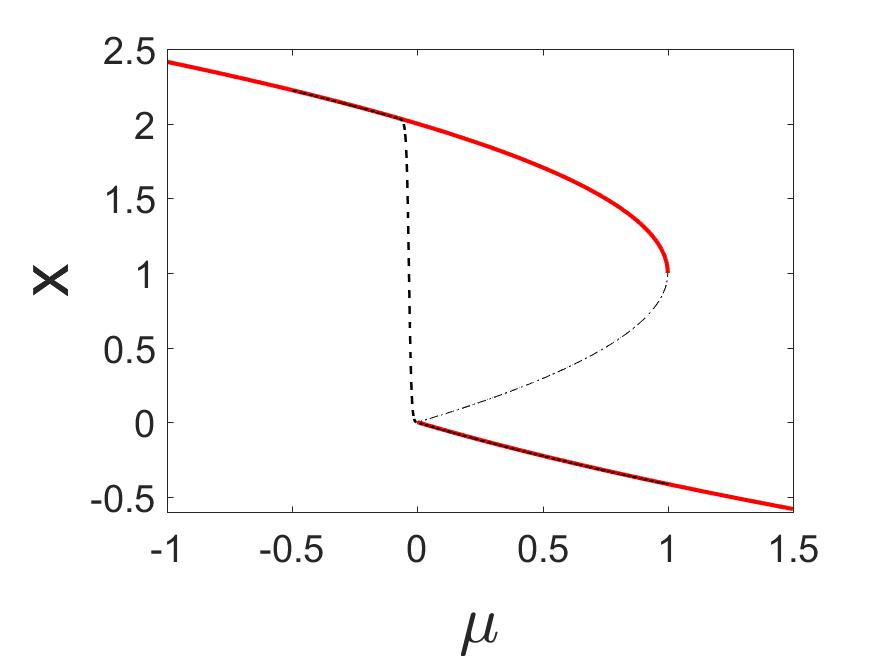
\includegraphics[width=\linewidth]{oneD/slowosc_bif_diagram_large.jpg}
 \caption{}
\end{subfigure}%
\begin{subfigure}{.5\textwidth}
 \centering
 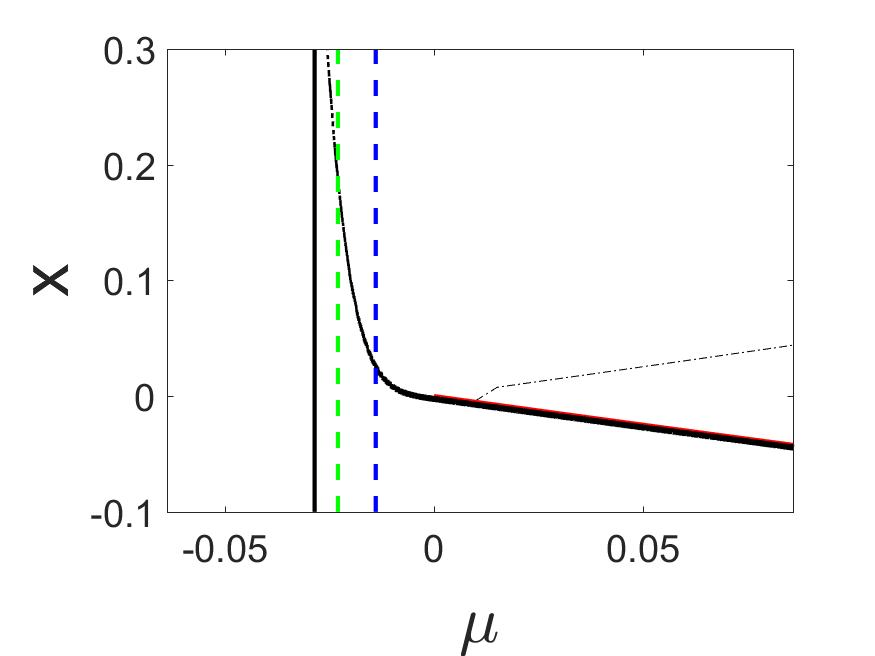
\includegraphics[width=\linewidth]{oneD/slowosc_bif_diagram_large_zoom.jpg}
 \caption{}
\end{subfigure}
\caption{Parameter values are $\epsilon=.05$, $\lambda=1.6$ and $A=4$. On the left, this is the bifurcation diagram for the 1D system with the numerical solution to \eqref{eq:oneD_canonical} (black dotted line). On the right, this is a zoom in. The dotted vertical lines are the tipping point $\mu_{\text{mixed}}$ \eqref{eq:oneD_slowosc_uglymu} (blue) and slowly varying tipping $\mu_{\text{slow}}$ \eqref{eq:oneD_slow_tipping} (green). The vertical line (black) is the numerically obtained tipping for $x>.5$.}
\label{fig:oneD_slowosc_numerical_large}
\end{figure}

In figure~\ref{fig:oneD_slowosc_lambdacomp} we compare the tipping between Case I and Case II with the numerical tipping. For smaller $\lambda$, the frequency $\Omega$ gets smaller and the Case I tipping becomes more predominant. But for the analysis performed in this section, $\Omega\gg 1$ and for $\lambda\le\frac{1}{2}$ we have $\Omega\sim O(1)$. We do not consider low frequency corresponding to $\lambda\le\frac{1}{2}$ in this section. The larger $\lambda$ becomes, the less effect we see from the oscillatory forcing until it is negligible for some $\lambda>1$. This is also seen in the asymptotic solution for each case, \eqref{eq:oneD_slowosc_outersoln}, \eqref{eq:oneD_slowosc_caseIsoln}, and \eqref{eq:oneD_slowosc_caseIIsoln} where the oscillatory component of the term has a $\epsilon^\lambda$ coefficient and shrinks the effects as $\lambda$ grows.

\begin{figure}[H]
\centering
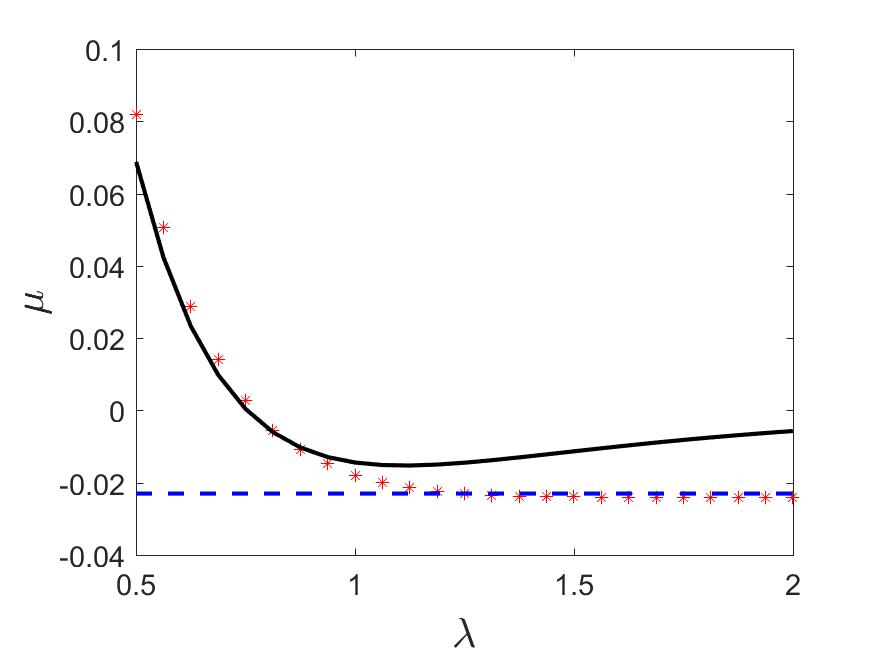
\includegraphics[width=0.7\textwidth]{oneD/slowosc_lambdacomp.jpg}
\caption{An example of numerical tipping (red stars) as the numerical solution to \eqref{eq:oneD_canonical} passes $x=.5$ for the last time. Parameter values are $\epsilon=.01$ and $A=4$. The lines are the Case I tipping estimate \eqref{eq:oneD_slowosc_uglymu} (black solid line) and the Case II tipping estimate \eqref{eq:oneD_slow_tipping} (blue dotted line).}
\label{fig:oneD_slowosc_lambdacomp}
\end{figure} 

The performance of our estimates are seen in figure~\ref{fig:oneD_slowosc_epscomp}. For Case I tipping, the range of appropriate $\epsilon$ is highly dependent on the choice in $\lambda$. Often, the range is very small to get accurate estimates. Both case approximations have good performance over a reasonable range of $\epsilon$.


\begin{figure}[H]
\centering
\begin{subfigure}{.5\textwidth}
 \centering
 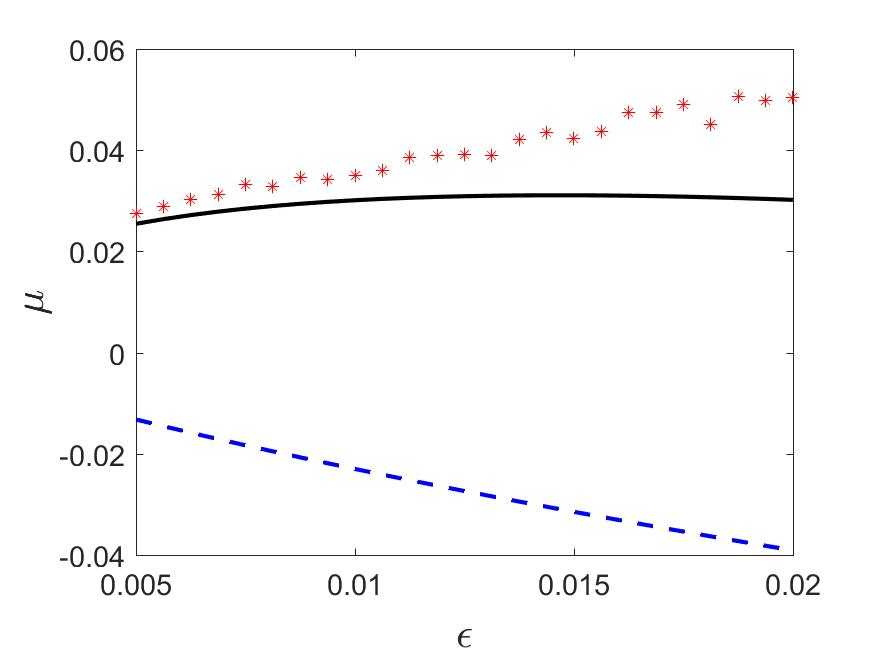
\includegraphics[width=\linewidth]{oneD/slowosc_epscomp_case2.jpg}
 \caption{$\lambda=.8$}
\end{subfigure}%
\begin{subfigure}{.5\textwidth}
 \centering
 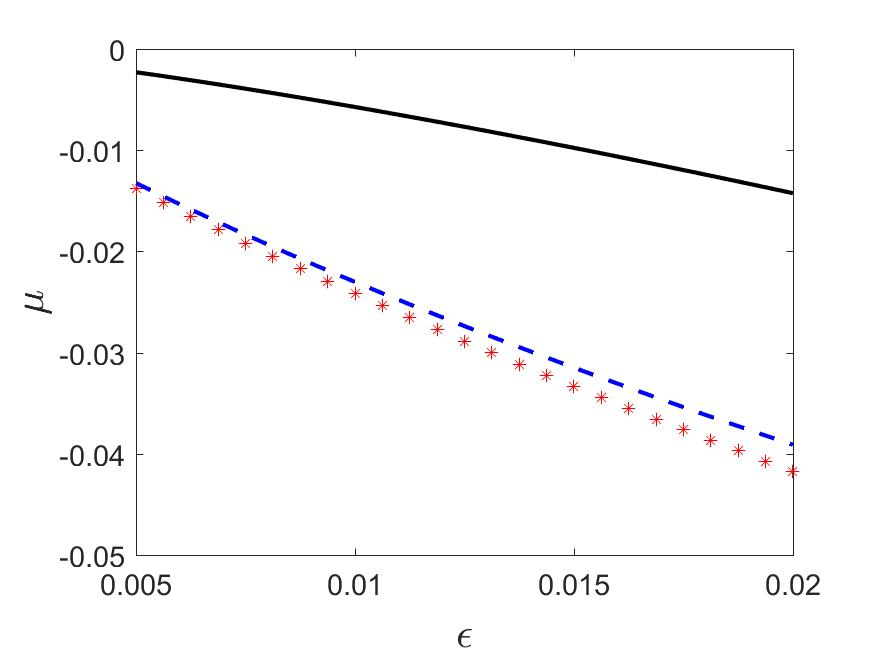
\includegraphics[width=\linewidth]{oneD/slowosc_epscomp_case3.jpg}
 \caption{$\lambda=1.3$}
\end{subfigure}
\caption{The numerical tipping (red stars) follows the appropriate case depending on $\lambda$. The Case I tipping estimate (black solid line) and the Case II tipping estimate (blue dotted line) are shown.}
\label{fig:oneD_slowosc_epscomp}
\end{figure}

\subsection{Stability}

Similarly to \autoref{sec:oneD_highfreqosc}, there are two ranges for $\lambda$ of interest that will govern the stability of solutions found in our analysis, $\lambda\le 1$ and $\lambda>1$.

\subsubsection{Case I: $\lambda\le 1$}

Recall for this case, we must have $\lambda\in (\frac{1}{2},1]$ and for this range, we found the inner equation

\begin{equation}\label{eq:oneD_slowosc_innerintegral}
{v_0}_t= -\epsilon^{1-\lambda}m(t)+\frac{1}{\pi}\int_0^{2\pi}| v_0(t)- A\cos(T)|\,dT=f(t,v_0).
\end{equation}

As in our analysis, we consider two regions of the solution $v_0(t)$ for this integral, in \autoref{subsec:oneD_slowosc_caseI} with Sub-Case I: $v_0(t)\le - |A|$ and in \autoref{subsec:oneD_slowosc_caseII} with Sub-Case II: $|v_0(t)|\le |A|$ where each these sub-cases deal with the respective size of $v_0(t)$ to the amplitude of the effective oscillations.

\subsubsection*{Sub-Case I: $v_0(t)\le - |A|$}

Recall from the analysis that the equation \eqref{eq:oneD_slowosc_innerintegral} simplifies in this region of $v_0(t)$ and has the following inner equation and pseudo-equilibrium

\begin{equation}\label{eq:oneD_slowosc_stabilitysubcaseI}
{v_0}_t= -\epsilon^{1-\lambda}m(t) -2v_0=f(t,v_0), \quad z^0(t)=-\epsilon^{1-\lambda}\frac{m(t)}{2}.
\end{equation}

As we saw in \autoref{sec:oneD_slow}, special treatment of the pseudo-equilibrium stability analysis is needed with linear perturbations $v_0(t)=z^0(t)+u(t)$ where $\lVert u(t)\rVert \ll 1$ and $z^0_t = -\epsilon^{1-\lambda}\frac{m_t}{2}=\frac{\epsilon^{1-\lambda}}{2}$. The resulting Taylor expansion is thus

\begin{equation*}
\begin{aligned}
{v_0}_t =& f(t,z^0)+f_{v_0}(t,v_0)(v_0(t)-z^0(t))+O(\lVert v_0(t)-z^0(t) \rVert^2),\\
u_t+z^0_t=&-2u+O(\lVert u(t)\rVert^2),\\
u_t =&-\frac{\epsilon^{1-\lambda}}{2}-2u.
\end{aligned}
\end{equation*}

This leads to the conclusion that equation \eqref{eq:oneD_slowosc_stabilitysubcaseI} causes perturbations to decay exponentially to a nearby equilibrium. Hence we find the pseudo-equilibrium to be hyperbolic and asymptotically stable.

\subsubsection*{Sub-Case II: $v_0(t)\le |A|$}

With the Taylor approximation from the analysis \eqref{eq:oneD_slowosc_subcaseIItaylor}, we have the following inner equation and pseudo-equilibrium

\begin{equation}\label{eq:oneD_slowosc_stabilitysubcaseII}
{v_0}_t= -\epsilon^{1-\lambda}m(t) +\frac{4|A|}{\pi}+\frac{2}{\pi |A|}v_0^2=f(t,v_0),\quad z^0(t)=-C \sqrt{\epsilon^{1-\lambda}m(t)-\frac{4|A|}{\pi}}
\end{equation}

We consider simple linear perturbations to this pseudo-equilibrium \eqref{eq:oneD_slowosc_stabilitysubcaseII}, $v_0(t)=z^0(t)+u(t)$ with $\lVert u(t) \rVert \ll 1$. Treating the pseudo-equilibrium carefully, we find that the slowly varying component of the equilibrium contributes to the derivative. Thus we have

\begin{equation}
\begin{aligned}
{v_0}_t =& z^0_t(t) +u_t,\\
z^0_t(t) = & \begin{cases}
\frac{\epsilon^{1-\lambda}}{2C\sqrt{\epsilon^{1-\lambda}m(t)-\frac{4|A|}{\pi}}} & \epsilon^{1-\lambda}m(t)> \frac{4|A|}{\pi},\\
0 & \epsilon^{1-\lambda}m(t) =\frac{4|A|}{\pi}.
\end{cases}
\end{aligned}
\end{equation}

Now applying a Taylor expansion, we find the following behavior of perturbations

\begin{equation}\label{eq:oneD_slowosc_stabilitysubcaseIIeq}
\begin{aligned}
{v_0}_t =& f(t,z^0)+f_{v_0}(t,z^0)(v_0-z^0(t))+O(\lVert v_0(t)-z^0(t) \rVert),\\
u_t =&\begin{cases}
-\frac{\epsilon^{1-\lambda}}{2C\sqrt{\epsilon^{1-\lambda}m(t)-\frac{4|A|}{\pi}}}-2\sqrt{\epsilon^{1-\lambda}m(t)-\frac{4|A|}{\pi}} u & \epsilon^{1-\lambda}m(t)>\frac{4|A|}{\pi},\\
0 & \epsilon^{1-\lambda}m(t)=\frac{4|A|}{\pi}.
\end{cases}
\end{aligned}
\end{equation}

From \eqref{eq:oneD_slowosc_stabilitysubcaseIIeq}, we find that the perturbations decay to a fixed negative quantity. This indicates, much like \autoref{sec:oneD_slow}, that there is an attracting equilibrium below the pseudo-equilibrium. The negative sign describes exponential decay and hence this equilibrium is hyperbolic and asymptotically stable for $\epsilon^{1-\lambda}m(t)>\frac{4|A|}{\pi}$ or $\mu(t)>\frac{4|A|}{\pi \Omega}$. But for $\epsilon^{1-\lambda}m(t)=\frac{4|A|}{\pi}$ or $\mu(t) =\frac{4|A|}{\pi \Omega}$, the stability of \eqref{eq:oneD_slowosc_stabilitysubcaseIIeq} suddenly becomes hyperbolic. This tells us that we lose stability at the oscillatory bifurcation but the tipping point occurs afterwards, which agrees with the conclusion in the tipping approximation from \eqref{eq:oneD_slowosc_caseItipping}.

\subsubsection{Case II: $\lambda>1$}

From the analysis, we discovered that for as long as $\epsilon^{\lambda-1}A\sim O(1)$, then we have very similar behavior in the tipping for this case. With the Taylor approximation from the analysis \eqref{eq:oneD_slowosc_caseII_integral}, the inner equation and pseudo-equilibrium is

\begin{equation}\label{eq:oneD_slowosc_stabilitycaseII}
\begin{aligned}
y_0=&-m(t) +\epsilon^{\lambda-1}\frac{2|A|}{\pi}+\epsilon^{1-\lambda}\frac{2}{\pi |A|}y_0^2=f(t,y),\\
z^0(t)=&-\epsilon^{\lambda-1}C\sqrt{m(t)-\epsilon^{\lambda-1}\frac{4|A|}{\pi}}.
\end{aligned}
\end{equation}

Similarly to Case I, we consider simple linear perturbations to this pseudo-equilibrium \eqref{eq:oneD_slowosc_stabilitycaseII}, $y_0(t)=z^0(t)+u(t)$ with $\lVert u(t) \rVert \ll 1$. Treating the pseudo-equilibrium carefully, we find that the slowly varying component of the equilibrium contributes to the derivative. Thus we have

\begin{equation}
\begin{aligned}
{y_0}_t =& z^0_t(t) +u_t,\\
z^0_t(t) = & \begin{cases}
\frac{\epsilon^{\lambda-1}}{2C\sqrt{m(t)-\epsilon^{\lambda-1}\frac{4|A|}{\pi}}} & m(t)> \epsilon^{\lambda-1}\frac{4|A|}{\pi},\\
0 & m(t) =\epsilon^{\lambda-1}\frac{4|A|}{\pi}.
\end{cases}
\end{aligned}
\end{equation}

Now applying a Taylor expansion, we find the following behavior of perturbations

\begin{equation}\label{eq:oneD_slowosc_stabilitycaseIIeq}
\begin{aligned}
{y_0}_t =& f(t,z^0)+f_{y_0}(t,z^0)(y_0-z^0(t))+O(\lVert y_0-z^0(t) \rVert^2),\\
u_t =&\begin{cases}
-\frac{\epsilon^{\lambda-1}}{2C\sqrt{m(t)-\epsilon^{\lambda-1}\frac{4|A|}{\pi}}}-2\sqrt{m(t)-\epsilon^{\lambda-1}\frac{4|A|}{\pi}} u & m(t)>\epsilon^{\lambda-1}\frac{4|A|}{\pi},\\
0 & m(t)=\epsilon^{\lambda-1}\frac{4|A|}{\pi}.
\end{cases}
\end{aligned}
\end{equation}

But the conclusions from Case I still apply to \eqref{eq:oneD_slowosc_stabilitycaseIIeq} and thus we still have stability up until $\mu(t)=\frac{4|A|}{\pi\Omega}$ and expect to see tipping occurring after the oscillatory bifurcation which is consistent with our tipping approximation for this case.

On the other hand, for large $\lambda$, the integral \eqref{eq:oneD_slowosc_caseII_integral} approaches

\begin{equation}\label{eq:oneD_slowosc_stabilitycaseII}
{y_0}_t=-m(t)+2|y_0|.
\end{equation}
But this is the same type of behavior from \autoref{sec:oneD_slow}, where we found that for $m(t)\ge 0$ our pseudo-equilibrium was stable and for $m(t)<0$ that searching for the pseudo-equilibrium causes a contradiction. Thus, we conclude that the tipping point occurs in the region of $m(t)<0$ which agrees with \eqref{eq:oneD_slow_tipping}.
